% \datum{06. November 2015}

\cite {L_BOOK},
\cite{bibel}

\section{Finite Elemente Methoden}
\label{sec:finite-elem-meth}

Anstelle der klassischen Formulierung
\begin{subequations}
  \label{eq:6-1}
  \begin{align}
    Lu = - \epsilon u'' - b u' + cu = f &\In (0, 1) = \Omega \label{eq:6-1a}\\
    u(0) = u(1) = 0 & \label{eq:6-1b}
  \end{align}
\end{subequations}
nutzen wir eine \markdef{schwache Formulierung}. Diese erhalten wir durch Nutzung des $L_{2}$-Skalarproduktes in Zusammenhang mit geeigneten Testfunktionen und geeigneten Testfunktionen und geeigneten Umformulierungen mithilfe der partiellen Integration. Es sei mit $(\cdot, \cdot)$ das $L_{2}$- Skalarprodukt über $(0, 1)$ gemeint. 
\begin{align*}
  - \int_{0}^{1} \epsilon u'' v - \int_{0}^{1} b u' v + \int_{0}^{1} cuv = \int_{0}^{1} fv\\
  \iff \quad - \epsilon (u'', v) - (bu', v) + (cu, v) = (f, v) \\
  - \epsilon (u'', v) = \epsilon (u', v') - \epsilon u'v|_{0}^{1}. 
\end{align*}
Einbindung der Randbedingungen \eqref{eq:6-1b}:
\begin{align*}
  u \in H_{0}^{1}(\Omega) = \set{u \in L_{2}(\Omega): \, u'\in L_{2}(\Omega), \, u|_{\pd \Omega} = 0},  
\end{align*}
$H_{0}^{1}$ ist ein Sobolevraum.

\paragraph{Exkurs}
Aus dem Sobolev-Einbettungssatz folgt: 

Für $k-j-\beta > \frac n2$ und $\Omega \subset \R^{n}$ gilt
\begin{align*}
  H^{k}(\Omega) \emb C^{j, \beta}(\bar \Omega)
\end{align*}
(Raum der Funktionen der Funktionen, deren $k$-te Ableitungen in $L_{2}$ liegen ist einbettbar in den Raum der Hölderstetigen Funktionen mit $\beta$). $k =1$, $n = 1$, $\beta = 0$, $j = 1$, also $1 - 0- 0 = 1 > \frac 12$. 
Also: Funktionen aus dem $H_{0}^{1}$ sind stetig. 

Exkurs Ende. 

Norm in $H_{0}^{1}(\Omega)$:
\begin{align*}
  \nnorm u_{1}^{2} \coloneqq   \nnorm {u'}_{0}^{2} +   \nnorm u_{0}^{2}
\end{align*}
mit der $H_{1}$-Seminorm $  \nnorm {u'}_{0}^{2}$ (ist schon eine Norm in $H_{0}^{1}$). 

Damit  $- \epsilon u' v |_{0}^{1}$ verschwindet, wählen wir $v \in H_{0}^{1}(\Omega)$. 

\paragraph{Schwache Formulierung} Gesucht: $u \in H_{0}^{1}(\Omega)$ mit
\begin{align}\label{eq:6-2}
  a(u, v)\coloneqq \epsilon(u', v') - (bu', v) + (cu, v) = (f, v) \quad \forall v \in H_{0}^{1}(\Omega). 
\end{align}
Beachte: \eqref{eq:6-1} $\implies$ \eqref{eq:6-2} $\stackrel {u \in C^{2}} \implies$ \eqref{eq:6-1}. Nicht jede Lösung von \eqref{eq:6-2} löst auch \eqref{eq:6-1}! Lösung für \eqref{eq:6-2} reicht uns allerdings\dots

Von nun an: $\nnorm \cdot _{0} = \nnorm \cdot_{L_{2}}$. 

\paragraph{Eigenschaften von $a(\cdot, \cdot)$}
\begin{enumerate}
\item $a(\cdot, v)$ und $a(u, \cdot)$ sind Funktionale, daher wird $a(\cdot, \cdot)$ \markdef{Bilinearform} genannt. 
\item Koerzitivität / $v$-Elliptizität:
  \begin{align*}
    a(u, u) &=\epsilon (u', u') - (bu', u) + (cu, u)\\
    - (bu', u) &= (u, (bu')) - \underbrace{ubu|_{0}^{1}}_{= 0} = (b'u, u) + (u, bu')\\
    \implies \quad - (bu', u) &= \(\frac 12 b'u, u\)
  \end{align*}
  Für $c + \frac 12 b' \geq \gamma > 0$ folgt
  \begin{align*}
    a(u, u) =& \epsilon (u', u') + ((c + \frac 12 b')u, u)\\
    &\geq \epsilon \nnorm{u'}_{L_{2}}^{2} + \gamma \nnorm{u}_{L_{2}}^{2} \eqqcolon \nnnorm u_{\epsilon}^{2}, 
  \end{align*}
  die \markdef{Energie-Norm}, $\epsilon$-gewichtete $H^{1}$-Norm. 
\item Stetigkeit
  \begin{align*}
    \norm{a(u, v)} &\leq \epsilon \nnorm {u'}_{L^{2}} \cdot \nnorm {v'}_{L^{2}} + \nnorm b_{L_{\infty}} \cdot \nnorm {u'}_{L^{2}} \cdot \nnorm {v}_{L^{2}} + \nnorm c_{L_{\infty}} \cdot\nnorm {u}_{L^{2}} \cdot \nnorm {v}_{L^{2}}\\
    &\leq \nnnorm u_{\epsilon} \cdot \nnnorm v_{\epsilon} + \gamma^{- \frac 12}\nnorm b_{L_{\infty}} \epsilon^{-\frac 12} \nnnorm u_{\epsilon} \nnnorm v_{\epsilon} + \frac 1 \gamma \nnorm c_{L_{\infty}} \cdot \nnnorm u_{\epsilon} \cdot \nnnorm v _{\epsilon}\\
    &\leq C(1 + \epsilon^{-\frac 12})\cdot\nnnorm u_{\epsilon}\cdot\nnnorm v_{\epsilon}
  \end{align*}
  Also ist $a(\cdot, \cdot)$ eine koerzitive, stetige Bilinearform, aber keine gleichmäßig stetige (das ist an mancher Stelle schlimm!). 
\end{enumerate}
\begin{bemerkung*}
  \begin{enumerate}
  \item   Es kann immer erreicht werden, dass
    \begin{align*}
      c + \frac 12 b' \geq \gamma > 0
    \end{align*}
    erfüllt ist, mittels einer Koordinatentransformation $u(x) = e^{\kappa \cdot x} v(x)$ mit geeignetem $\kappa$. 
  \item Ist die Norm $\nnnorm \cdot_{\epsilon}$ sinnvoll? In  $\nnnorm \cdot_{\epsilon}$ ist \eqref{eq:6-1} singulär gestört, da
    \begin{align*}
      \nnnorm {e^{- \beta \frac x \epsilon}}_{\epsilon} &\geq\epsilon^{\frac 12}\cdot \nnorm{e^{-1} e^{- \beta \frac x \epsilon}}_{L_{2}} = \cO(1)
    \end{align*}
    (bezüglich $\epsilon$ konstant!!) Es folgt, dass
    \begin{align*}
      \lim_{\epsilon \to 0}    \nnnorm {e^{- \beta \frac x \epsilon}}_{\epsilon}  > 0
    \end{align*}
    und damit ist das Problem auch bezüglich $\nnnorm \cdot _{\epsilon}$ singulär gestört. 
  \end{enumerate}
\end{bemerkung*}
\begin{lemma}\label{lem:6-1} Lax-Milgram
  Die Variationsgleichung \eqref{eq:6-2} besitzt für jedes $f \in L_{2}(\Omega)$ (sogar $(H_{0}^{1}(\Omega))' = H^{-1}$) eine eindeutige Lösung $u \in H_{0}^{1}(\Omega)$. 
\end{lemma}
\begin{beweis}
  Banach'scher Fixpunktsatz und so weiter\dots
\end{beweis}
\begin{bemerkung*}
  Mit der Koerzitivität und der Stetigkeit folgt
  \begin{align*}
    \nnnorm u_{\epsilon}^{2} &\leq a(u, u) = (f, u) \leq \nnorm f_{L_{2}} \cdot \nnorm u_{L_{2}} \leq \frac {\nnorm f_{L_{2}}}{\gamma^{\frac 1 2}} \nnnorm u_{\epsilon}\\
    \implies \quad \nnnorm u_{\epsilon} &\leq \gamma^{-\frac 1 2} \nnorm f_{L_{2}}
  \end{align*}
  (Lösung ist in der Energienorm beschränkt). Aber es ist eine \emph{schlechte} Schranke! 
\end{bemerkung*}

\paragraph{Diskretisierung}
Wählen wir $U_{h}\subset H_{0}^{1}(\Omega)$ und $V_{h}\subset H_{0}^{1}(\Omega)$ endlichdimensional, so erhalten wir für $U_{h} \neq V_{h}$ die \markdef{Petrov-Galerkin-Methoden}: 
\begin{center}
  Gesucht: $u_{h}\in U_{h}$ mit $ a(u_{h}, v_{h}) = (f, v_{h})$ für alle $v_{h} \in V_{h}$ 
\end{center}
und für $U_{h} = V_{h}$ die \markdef{Galerkin-Methoden} (hier im Wesentlichen betrachtet)
\begin{center}
  Gesucht: $u_{h}\in V_{h}$ mit $ a(u_{h}, v_{h}) = (f, v_{h})$ für alle $v_{h} \in V_{h}$. 
\end{center}
Mit einer Basis $\set{\phi_{i}}_{i = 1}^{M}$ von $ V_{h} = U_{h}$ folgt für die Galerkin-Methode
\begin{align*}
  u_{h} = \sum_{i = 1}^{M} u_{i} \phi_{i}
\end{align*}
und aus $a(u_{h}, v_{h}) = (f, v_{h})$ wird
\begin{align*}
  \sum_{i = 1}^{M} u_{i} a(\phi_{i}, \phi_{j}) &= (f, \phi_{j}) \quad j = 1, \dots, M\\
  \iff \qquad A U &= F
\end{align*}
mit $A = (a_{ij})$ mit $a_{ij} = a(\phi_{j}, \phi_{i})$, $F = \((f, \phi_{j})\)_{j = 1}^{M}$. Das ist ein Lineares Gleichungssystem. Das Lösungsverhalten des numerischen Lösers hängt von der Basis $\set{\phi_{i}}$ ab. Optimale Basis: $a(\phi_{i}, \phi_{j}) = \delta_{ij}$, aber dies ist im Allgemeinen nicht praktikabel, da die $\set{\phi_{i}}$ Lösungen des Originalproblems sein müssten. Daher wählt man eine Basis, in der nicht jede Funktion mit jeder interagiert. Also ist $A$ dünn besetzt. 

\paragraph{Gitter}
Sei dazu ein Gitter $\omega$ mit $0 = x_{0} \leq \dots \leq x_{N} = 1$ gegeben. Wir erzeugen uns eine Funktionsfolge aus $C^{0}$-Polynomsplines. 

\paragraph{Lineare Elemente} ($C^{0}$-$P_{1}$-Spline, $S^{1} = S_{0}^{1}$ (Splines), Hütchenfunktionen, \dots) $\phi_{i}$ ist stückweise linear und $\phi_{i}(x_{j}) = \delta_{ij}$, also
\begin{align*}
  \phi_{i}(x) =
  \begin{cases}
    \frac{x - x_{i-1}}{x_{i} - x_{i-1}}, & x \in[x_{i - 1}, x_{i}]\\
    \frac{x_{i+1} - x}{x_{i+1} - x_{i}}, & x \in[x_{i}, x_{i+1}]\\
    0, & \text{sonst}. 
  \end{cases}
\end{align*}
Also $a (\phi_{i}, \phi_{j}) = 0$ für $\norm{i-j} > 1$, also ist $A$ tridiagonal. Lösen von $AU = F$ kostet $\cO(N)$ mit dem Thomas-Algorithmus. 

\paragraph{Elemente höherer Ordnung}
Lokale Sichtweise (für ein Intervall $[x_{i-1}, x_{i}]$): Wir definieren einen geeigneten lokalen Polynomraum.
\begin{enumerate}
\item Hierarchische Basis, linear: lokal $\Pi_{1}$; linear mit quadratischer Blasenfunktion: lokal $\Pi_{2}$; zusätzlich kubisch: lokal $\Pi_{3}$ und so weiter. 

  Lineare Funktionen müssen stetig verknüpft werden, damit $V_{h} \subset H_{0}^{1}(\Omega)$ und der Rest sind stetige Blasenfunktionen. Weiterhin haben wir eine Matrix mit Bandstruktur. Dann ist ($P$ ist maximaler Polynomgrad)
  \begin{align*}
    u_{h} =  \sum_{i = 1}^{N-1} u^{1}_{i} \underbrace{\phi_{i}^{1}}_{\text{lin. Hütchenfkt.}} + \sum_{i = 1}^{N} \sum_{j = 2}^{P} u_{i}^{j} \underbrace{\phi_{i}^{j}}_{\text{lokale Blase, Grad }j}
  \end{align*}

\item Standard-Lagrange-Basis
\end{enumerate}
% \datum{12. November 2015}

\begin{beispiel}\label{ex:6-2}
  Galerkin-FEM mit linearen Ansatzfunktionen über einem äquidistanten Gitter
  \begin{align*}
    h_{i} &= \frac 1N \eqqcolon h\\
    \phi_{i} &=
    \begin{cases}
      \frac{x - x_{i-1}} h, & x \in(x_{i-1}, x_{i})\\
      \frac{x_{i+1} - x} h, & x \in(x_{i}, x_{i+1})\\
      0, & \text{sonst}
    \end{cases}
  \end{align*}
  Integrale in $(a(u_{h}, \phi_{j})) = (f, \phi_{j})$ werden üblicherweise mittels einer Quadraturformel berechnet. Sei diese die Mittelpunktregel, das heißt
  \begin{align*}
    \int_{x_{i-1}}^{x_{i}} f(x) dx\approx h\cdot f\(x_{i - \frac 12}\). 
  \end{align*}
  Dann erhalten wir ein lineares Gleichungssystem der Form
  \begin{align*}
    - \epsilon [D^{2}u]_{i} + \frac 12 \(b_{i-\frac 12} [D^{-}u]_{i}  + b_{i+ \frac 12}[D^{+}u]_{i}\) + \frac 12 \( c_{i- \frac 12} + c_{i+ \frac 12}\)u_{i} \\
    &= \frac 12 \( f_{i- \frac 12} + f_{i+ \frac 12}\)
  \end{align*}
  mit
  \begin{align*}
    [D^{+}u]_{i} &\coloneqq \frac{u_{i+1} - u_{i}} h\\
    [D^{-}u]_{i} &\coloneqq \frac{u_{i} - u_{i-1}} h\\
    [D^{2}u]_{i} &\coloneqq [D^{+} D^{-} u]_{i}
  \end{align*}
  Dies ist ein Differenzenverfahren und für $b, c, f$ konstant ist dies das klassische zentrale Differenzenverfahren:
  \begin{align*}
    - \epsilon \frac{u_{i+1} - 2 u_{i} + u_{i-1}}{h^{2}} + b \frac{u_{i+1}-u_{i-1}}{2\cdot h} + c\cdot u_{i} = f_{i}
  \end{align*}
  =(. 
\end{beispiel}

\paragraph{Klassische Fehleranalysis}
Sei dazu $P: H_{0}^{1}(0, 1) \to V_{h}$ eine Projektion, zum Beispiel Interpolation. Dann gilt
\begin{enumerate}
\item \label{num:i} die Galerkin-Orthogonalität
  \begin{align*}
    a(u - u_{h}, \phi_{j}) = 0 \quad \forall \phi_{j}\in V_{n};
  \end{align*}
\item \label{num:ii}mithilfe der Koerzitivität:
  \begin{align*}
    \nnnorm{u-u_{h}}_{\epsilon}^{2} &\leq a(u-u_{h}, u- u_{h})\\
    &= a(u-u_{h}, u-u_{h}+ \underbrace{u_{h} - Pu}_{= 0, \, \in V_{h}})\\
    &= a(u-u_{h}, u- Pu)\\
    &\leq C\cdot \nnnorm{u-u_{h}}_{\epsilon} \cdot\nnnorm{u-Pu}_{\epsilon} + C\cdot \epsilon^{-\frac 12} \nnnorm{u-u_{h}}_{\epsilon}\cdot\nnnorm{u-Pu}_{\epsilon}
  \end{align*}
  mit Stetigkeit und \ref{num:i}. Wir erhalten
  \begin{align*}
    \nnnorm{u-u_{h}}_{\epsilon} &\leq  C\cdot \epsilon^{-\frac 12} \cdot \nnnorm{u-Pu}_{\epsilon}
  \end{align*}
  (Version des Lemmas von Cea, Quasi-Optimalität bezüglich der $\nnnorm\cdot_{\epsilon}$). 
\end{enumerate}
Angenommen, $P$ ist eine nodale Interpolierende, das heißt, $Pu(x_{i}) = u(x_{i})$, $i = 0, \dots, N$, dann
\begin{align*}
  \nnnorm{u-Pu}_{\epsilon} \leq \epsilon^{\frac 12}\nnorm{(u-u^{I})'}_{L_{2}} + \gamma \nnorm{u-u^{I}}_{L_{2}}. 
\end{align*}
Mit $u \in H^{2}(0, 1) = \set{u \in L_{2}: \,  u', u'' \in L_{2}}$ folgt
\begin{align*}
  \nnnorm{u - Pu}_{\epsilon} &\leq \epsilon^{\frac 12} C H\norm u_{2} + CH^{2} \nnorm u_{2}\\
  &\leq C(\epsilon^{\frac 12} + H) H\norm u_{2} \\
  \norm{u''(x)}\leq C(1 + \epsilon^{-2}e^{- \beta \frac x \epsilon}) \implies \norm u_{2} \leq C\cdot\epsilon^{- \frac 32}\\
  \implies \nnnorm{u-u_{h}}_{\epsilon} \leq C \cdot \epsilon^{- \frac 12}(\epsilon^{\frac 12} + H)\cdot H\cdot \epsilon^{- \frac 32}\\
  \leq C \cdot H\cdot \epsilon^{- \frac 32}(1 + \epsilon^{-\frac 12} + H)
\end{align*}
($\norm \cdot_{2}$ ist die Norm in $H^2$, $\norm v_{2} = \nnorm {v''}_{L_{2}}$). 
Das ist keine gleichmäßige Konvergenz! Auswege:
\begin{enumerate}
\item verbesserte Analysis (immer notwendig!)
\item angepasste Funktionenräume (entweder \dots)
\item angepasste Gitter (\dots oder)
\item Stabilisierungsmethoden (optional, in Kombination)
\end{enumerate}

\subsection{Angepasste Funktionenräume}
\label{sec:angep-funkt}

Mit Hilfe der Greenschen Funktion $G$, die Lösung von
\begin{align*}
  L^{*}G(x, \zeta) = - \epsilon G'' + (bG)' + cG &= \delta(\zeta-x)\\
  G(x, 0) = G(x, 1) &= 0
\end{align*}
mit $(Lv, G) = (v, L^{*}G)$ erhalten wir eine Lösungsdarstellung
\begin{align*}
  u(x) = \int_{0}^{1}f(t) G(x, t)dt. 
\end{align*}
Nützlich für Theorie, Praxis weniger. 
($G$ erfüllt auch
\begin{align*}
  LG(x, \zeta) = - \epsilon G'' - bG' + cG &= \delta(x - \zeta)\\
  G(0, \zeta) = G(1, \zeta) &= 0. )
\end{align*}
Speziell folgt
\begin{align*}
  u(x_{i}) &= \int_{0}^{1}f(t) G(x_{i}, t)dt\\
  &= \int_{0}^{1}(Lu)(t) G(x_{i}, t) dt\\
  &= \int_{0}^{1}u(t) L^{*}G(x_{i}, t) dt\\
  &= a (u, G(x_{i}))
\end{align*}
($G(x_{i})$ sei Testfunktion). 
Also sind gute Testfunktionen solche, die $G_{i} = G(x_{i}, \cdot)$ approximieren. Diese Idee stammt von Hemker (1977).  Dies motiviert die Definition der \markdef{$\bar L^{*}$-Splines} oder \markdef{Hemker-Funktionen} $\psi_{i} \in H_{0}^{1}$ (Kombination von $\exp$-Funktionen), $i= 1, \dots, N-1$, die per
\begin{enumerate}
\item $\bar L^{*} \psi_{i} = - \epsilon \psi_{i}'' + \bar b \psi_{i}' + \bar c \psi_{i} = 0$
  auf jedem $x_{j-1}, x_{j}$, $j = 1, \dots, n$
\item $\psi_{i}(x_{j}) = \delta_{ij}$, $j = 0, \dots, n$
\end{enumerate}
definiert sind, wobei $\bar b$ und $\bar c$ stückweise konstante Approximiationen von $b$ und $c$ sind. 

\begin{figure}[bht!]
  \centering
  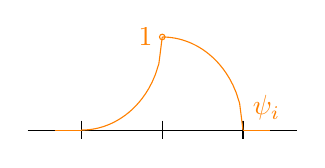
\begin{tikzpicture}

    \begin{axis}[ymin = -.1, ymax = 1.1, xmin= -2, xmax=8, axis y line = none, axis x line = none, height = 3cm, width = 5cm]
      \draw (axis cs:-2, 0) -- (axis cs:8, 0);
      \draw (axis cs:0, 0.1) -- (axis cs:0, -0.1) node[below] at (axis cs:0, -0.1) {$x_{i-1}$};
      \draw (axis cs:3, 0.1) -- (axis cs:3, -0.1) node[below] at (axis cs:3, -0.1) {$x_{i}$};
      \draw (axis cs:6, 0.1) -- (axis cs:6, -0.1) node[below] at (axis cs:6, -0.1) {$x_{i+1}$};

      \addplot[orange, domain = 0:3] {1 - sqrt(9 - x^2)*1/3};
      \addplot[orange, domain = 3:6] {sqrt(9 - (x- 3)^2)*1/3} node[above right] {$\psi_{i}$};
      \addplot[orange, domain = -1:0] {0};
      \addplot[orange, domain = 6:7] {0};
      \draw[orange](axis cs: 3, 1)circle (1pt) node[left] {$1$};
    \end{axis}    
  \end{tikzpicture}
  \caption{Haifischflosse, $\bar L^{*}$-Splines}
  \label{fig:hai}
\end{figure}


Sei außerdem die diskretisierte Green'sche Funktion $G_{i}(x)$ definiert als
\begin{enumerate}
\item $- \epsilon G_{i}'' + \bar b G_{i}' + \bar c G_{i} = 0$ auf jedem $(x_{j-1}, x_{j})$, $j = 1, \dots, n$, 
\item $G_{i} \in C[0, 1]$ mit $G(0) = G(1) = 0$, 
\item \label{num:iii} $\lim_{x \to x_{j}^{-0}} (\epsilon G_{i}' - \bar b G_{i})(x) - \lim_{x \to x_{j}^{+0}} (\epsilon G_{i}' - \bar b G_{i})(x) = \delta_{ij}$
%  skizze 2  

\end{enumerate}
Also $G_{i} \in \set{\bar L^{*} - \text{Spline}}$ und $\nnorm {G_{i}}_{L_{\infty}}\leq C$. Wir brauchen noch eine passende Bilinearform: 

Sei
\begin{align*}
  \bar a (u, v)\coloneqq \epsilon (u', v') + (\bar c u - \bar b u', v). 
\end{align*}
\begin{satz}\label{thm:6-3}
  Sei $V_{h} = \set{\bar L^{*} - \text{Spline}}$ und $U_{h} = \set{\text{stückweise linear}}$. 
  Dann gilt für $u_{h} \in U_{h}$ mit
  \begin{align*}
    \bar a(u_{h}, v_{h}) = (\bar f, v_{h})\quad \forall v_{h} \in V_{h}, 
  \end{align*}
  dass
  \begin{align*}
    \norm{u(x_{i}) - u_{i}} \leq C\cdot H, \quad i = 1, \dots, n-1, \, H = \max_{i} h_{i}. 
  \end{align*}
\end{satz}
\begin{beweis}
  Sei $i \in \set{1, \dots, n-1}$ fest. Für jedes $w \in H_{0}^{1}(0, 1)$ gilt
  \begin{align*}
    \bar a(w, G_{i}) &= \epsilon (w', G_{i}') + (\bar c w + \bar b w', G_{i})\\
    &= (w', \epsilon\cdot  G_{i}' - \bar b G_{i}) + (\bar c w, G_{i})\\
    &\stackrel{\ref{num:iii}} = \sum_{j = 1}^{N} \int_{x_{j-1}}^{x_{j}} w(x) (-\epsilon G_{i}'' + \bar b G_{i}')(x) dx + w(x_{i}) + (\bar c w, G_{i})\\
    & = \sum_{j = 1}^{N} \int_{x_{j-1}}^{x_{j}}  \underbrace{(-\epsilon G_{i}'' + \bar b G_{i}' + \bar c G_{i})}_{\stackrel{\ref{num:i}}= 0}(x)  w(x)dx + w(x_{i})  = w(x_{i}), 
  \end{align*}
  macht also diskret dasselbe, wie die Green'sche Funktion. Daher der Name 'diskretisierte Green'sche Funktion'. Also folgt
  \begin{align*}
    u(x_{i}) - u_{i} &= \bar a (u - u_{h}, G_{i})\\
    &= \bar a (u, G_{i}) -\bar a (u_{h}, G_{i}) \quad G_{i} \in V_{h}\\
    &= \bar a (u, G_{i}) - (\bar f , G_{i}) \\
    &= \bar a (u, G_{i}) - a(u , G_{i}) + a(u , G_{i})  - (\bar f, G_{i})\\
    &= \bar a (u, G_{i}) - a(u , G_{i}) +( f - \bar f, G_{i})\\
    &= - ((b - \bar b)u', G_{i}) + ((c-\bar c) u, G_{i}) + ( f - \bar f, G_{i}). 
  \end{align*}
  Mit $\norm{b - \bar b} \leq C\cdot H$, $\norm{c - \bar c} \leq C\cdot H$, $\norm{f - \bar f} \leq C\cdot H$, $\nnorm{G_{i}}_{L_{\infty}}\leq C$, $\nnorm{u}_{L_{\infty}}\leq C$ und $\nnorm{u'}_{L_{1}}\leq C$ folgt die Aussage. 
\end{beweis}
\begin{bemerkung*}
  Auf einem äquidistanten Gitter mit $\bar z|_{(x_{i-1}, x_{i})} = z_{i - \frac 12}$ oder $\bar z|_{(x_{i-1}, x_{i})} = \frac 12 (z_{i-1} + z_{i})$ für $z = b, c, f$ erzeugt dieses Petrov-Galerkin-Verfahren ein Differnzenschema, welches auch als ElMistikawy-Werle-Schema bekannt ist. Der Konvergenzbeweis kann mit schwierigeren Mitteln auf
  \begin{align*}
    \norm{u(x_{i}) - u_{i}} \leq C\cdot H^{2}
  \end{align*}
  verbessert werden (siehe Bibel, alte Version ).
\end{bemerkung*}
Im Allgemeinen gilt trotzdem in der ersten Gitterzelle
\begin{align*}
  \max_{x \in (0, x_{1})} \norm{u(x) - u_{h}(x)} = \cO(1), \qquad H \gg\epsilon. 
\end{align*}
=(
% (skizze 3)

% 'Hier fehlt noch was'. 

Trotz 'guter' Methode erhalten wir nur in den Gitterpunkten eine gute Lösung. Außerhalb dieser (speziell im Grenzschichtbereich) ist der Approximationsfehler mit stückweise linearen Funktionen zu schlecht. Wir sollten also einen Raum nutzen, der das Lösungsverhalten besser wiederspiegelt (andere Funktionen verwenden). 

Die natürliche Wahl sind hier die $\bar L$-Splines $\Span \set{\phi_{i}}_{i = 1}^{N-1}$ mit
\begin{align*}
  \bar L \phi_{i} = - \epsilon \phi_{i}''  - \bar b \phi_{i}' + \bar c \phi_{i} = 0
\end{align*}
auf jedem $(x_{j-1}, x_{j})$, $j = 1, \dots, n$, $\phi_{i}(x_{j}) = \delta_{ij}$, $j = 1, \dots, n$. 

\begin{figure}[bht!]
  \centering
  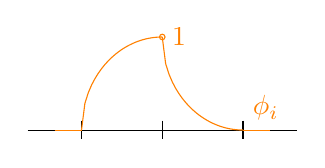
\begin{tikzpicture}

    \begin{axis}[ymin = -.1, ymax = 1.1, xmin= -8, xmax=2, axis y line = none, axis x line = none, height = 3cm, width = 5cm]
      \draw (axis cs:-8, 0) -- (axis cs:2, 0);
      \draw (axis cs:-6, 0.1) -- (axis cs:-6, -0.1) node[below] at (axis cs:-6, -0.1) {$x_{i-1}$};
      \draw (axis cs:-3, 0.1) -- (axis cs:-3, -0.1) node[below] at (axis cs:-3, -0.1) {$x_{i}$};
      \draw (axis cs:0, 0.1) -- (axis cs:0, -0.1) node[below] at (axis cs:0, -0.1) {$x_{i+1}$};

      \addplot[orange, domain = -6:-3] {sqrt(9 - (x+3)^2)*1/3};
      \addplot[orange, domain = -3:0] {1 - sqrt(9 - x^2)*1/3}node[above right] {$\phi_{i}$};
      \addplot[orange, domain = -7:-6] {0};
      \addplot[orange, domain = 0:1] {0};
      \draw[orange](axis cs: -3, 1)circle (1pt) node[right] {$1$};
    \end{axis}    
  \end{tikzpicture}
  \caption{Inverse Haifischflosse, $\tau$-Spline}
  \label{fig:hai2}
\end{figure}
% \datum{13. November 2015}

\begin{bemerkung*}
  Für $\chi \in \set{\bar L\text{-Splines}}$ gilt
  \begin{align*}
    \nnorm{\chi'}_{L_{1}(x_{i-1}, x_{i})} \leq C\cdot h_{i}^{- \frac 12} \epsilon^{\frac 12}\nnorm{\chi'}_{L_{2}(x_{i-1}, x_{i})}
  \end{align*}
  (siehe \cite{OS_MC}). 
\end{bemerkung*}
\begin{lemma}\label{lem:6-4}
  Auf einem äquidistantem Gitter $x_{0}< x_{1}< \dots < x_{N}$ sei der Raum $U_{h} = \set{\bar L\text{-Splines}}$ gegeben und mit $u^{I}$ bezeichnen wir die nodale Interpolierende aus $U_{h}$, das heißt
  \begin{align*}
    u^{I}(x_{i}) = u(x_{i}) \quad \forall i. 
  \end{align*}
  Dann gilt
  \begin{enumerate}
  \item \begin{align*}
      \nnorm{u-u^{I}}_{L_{\infty}} &\leq C\cdot H, 
    \end{align*}
  \item
    \begin{align*}
      \nnnorm{u-u^{I}}_{\epsilon} &\leq  C\cdot H^{\frac 12}. 
    \end{align*}
  \end{enumerate}
\end{lemma}
\begin{beweis}
  \begin{enumerate}
  \item   Vergleichsprinzip mit $S(x) = C(x - x_{i-1})$ auf jedem Teilinterval. 
  \item Nun zur Energienorm:
    \begin{align*}
      \nnnorm{u-u^{I}}^{2}_{\epsilon} &\leq a(u-u^{I}, u-u^{I})\\
      &= \sum_{i} \int_{x_{i-1}}^{x_{i}} \( - \epsilon(u-u^{I})'' - b(u-u^{I})' + c(u- u^{I})\)(u-u^{I}) dx\\
      &= \sum_{i} \int_{x_{i-1}}^{x_{i}} \(\underbrace{Lu}_{= f} - \underbrace{\bar L u^{I}}_{= 0} + ' (b- \bar b)(u^{I})' + (c- \bar c)(u^{I})\)(u-u^{I}) dx
\end{align*}
\begin{align*}
      &\norm{ \sum_{i} \int_{x_{i-1}}^{x_{i}} \(f - (c- \bar c)(u^{I})\)(u-u^{I}) dx} \\
&\quad\leq \(\nnorm f_{L_{\infty}} + 2\cdot\nnorm c _{L_{\infty}}\nnorm{u^{I}}_{L_{\infty}}\) \underbrace{\sum_{i} \int_{x_{i-1}}^{x_{i}} \nnorm{u-u^{I}} dx}_{\leq C\cdot H}\\
      &\norm{ \sum_{i} \int_{x_{i-1}}^{x_{i}} \(b - \bar b\)(u^{I})(u-u^{I}) dx}  \\
&\quad\leq\sum_{i} \nnorm{(u^{I})'}_{L_{1}(x_{i-1}, x_{i})} \cdot \underbrace{\nnorm{b - \bar b}_{L_{\infty}(x_{i-1}, x_{i})}}_{\leq C\cdot \nnorm{b'}_{L_{\infty}(x_{i-1}, x_{i})}\cdot h_{i}} \cdot \nnorm{u - \bar u^{I}}_{L_{\infty}(x_{i-1}, x_{i})}\\
      &\quad\leq C\cdot \nnorm{u - u^{I}}_{L_{\infty}} \cdot \nnorm{b'}_{L_{\infty}} \cdot \sum_{i} h_{i} h_{i}^{- \frac 12} \epsilon^{\frac 12} \nnorm{(u^{I})'}_{L_{2}(x_{i-1}, x_{i})}\\
      &\quad\leq C\cdot \nnorm{u - u^{I}}_{L_{\infty}} \cdot \nnorm{b'}_{L_{\infty}} \cdot \epsilon^{\frac 12}\underbrace{\(\sum_{i} h_{i}\)^{\frac 12}}_{= 1} \(\sum_{i} \nnorm{(u^{I})'}_{L_{2}(x_{i-1}, x_{i})}^{2}\)^{\frac 12}\\
      &\quad\leq C\cdot \nnorm{b'}_{L_{\infty}} \cdot \underbrace{\epsilon^{\frac 12} \cdot \nnorm{(u^{I})'}_{L_{2}}}_{\leq \nnnorm{u^{I}}_{\epsilon} \leq C} \nnorm{u- u^{I}}_{\infty}\leq C\cdot H. 
    \end{align*}
    per partieller Integration im ersten Schritt und später Hölder, mit
    \begin{align*}
      \nnorm{u^{I}}_{L_{\infty}}\leq \underbrace{\nnorm u_{L_{\infty}}}_{\leq C} + \underbrace{\nnorm{u-u^{I}}_{L_{\infty}}}_{C \cdot H}. 
    \end{align*}
  \end{enumerate}
\end{beweis}
Die Schranken in Lemma \ref{lem:6-4} sind scharf!
\begin{satz}\label{thm:6-5}
  Gegeben sei ein äquidistantes Gitter und die Galerkin-FEM mit $U_{h} = V_{h} = \set{\bar L\text{-Splines}}$. Gesucht ist $u_{h} \in U_{h}$ mit
  \begin{align*}
    \bar a (u_{h}, v_{h}) = (\bar f, v_{h}) \quad \forall v_{h} \in V_{h}. 
  \end{align*}
  Dann gilt
  \begin{align*}
    \nnnorm{u - u_{h}}_{\epsilon} \leq C\cdot H^{\frac 12}. 
  \end{align*}
\end{satz}
\begin{beweis}
  Es muss nur noch der diskrete Fehler $\nnnorm{u^{I} - u_{h}}_{\epsilon}$ abgeschätzt werden. Seien dazu vereinfacht $b$ und $c$ konstant. Dann gilt für $\chi = u^{I} - u_{h} \in V_{h}$. 
  \begin{align*}
    \nnnorm \chi^{2}_{\epsilon} &\leq a(u^{I} - u_{h}, \chi)\\
    &\leq a(u^{I} - u, \chi) + a (u - u_{h}, \chi)\\
    &\leq a(u^{I} - u, \chi) + a (u, \chi) - \bar a (u_{h}, \chi)\\
    &\leq a(u^{I} - u, \chi) + (f - \bar f, \chi)\\
    &\leq \epsilon\nnorm{(u^{I} - u)'}_{L_{2}} \nnorm {\chi'}_{L_{2}} + (b(u^{I}- u), \chi') + c\nnorm{u^{I} - u}_{L_{2}} \nnorm \chi_{L_{2}} + C \cdot H \nnorm \chi_{L_{2}}\\
    &\leq C\( H^{\frac 12} + H\) \nnnorm \chi_{\epsilon} + (b(u^{I}- u), \chi') \\
    &\leq C\( H^{\frac 12} + H\) \nnnorm \chi_{\epsilon} + b\nnorm{u^{I}- u}_{L_{\infty}} \cdot\underbrace{\nnorm{ \chi'}_{L_{1}} }_{H^{- \frac 12} \epsilon^{\frac 12} \nnorm{\chi'}_{L_{2}}}\\
    &\leq C\( H^{\frac 12} + H + H^{\frac 12}\) \nnnorm \chi_{\epsilon}
  \end{align*}
  mit Cauchy-Schwarz, Lemma \ref{lem:6-4}, Hölder und mehrfachem Ausnutzen der Tatsache, dass $b$ und $c$ konstant sind. Also
  \begin{align*}
    \nnnorm{u -u_{h}}_{\epsilon} \leq   \nnnorm{u -u^{I}}_{\epsilon} +   \nnnorm{u^{I} -u_{h}}_{\epsilon} \leq C \cdot H^{\frac 12}. 
  \end{align*}
\end{beweis}
Satz \ref{thm:6-3} besagt, dass das Paar $\bar L ^{*}$-Splines/stückweise Linear in der diskreten Norm $\nnorm \cdot_{\infty, d} = \max_{i} \norm{\cdot (x_{i})}$ mit  der Ordnung $1$ konvergiert. 

Satz \ref{thm:6-5} besagt, dass das Paar $\bar L$-Splines/$\bar L$-Splines in der Energienorm mit der Ordnung $\frac 12$ konvergiert. Beide Schranken sind scharf (nicht verbesserbar)!

\begin{bemerkung}\label{rem:6-6}
  Es seien $U_{h} = \set{\bar L\text{-Splines}}$ und $V_{h} = \set{z_{i}}_{i = 1}^{n-1}$ mit $z_i(x_{j}) = \delta_{ij}$ beliebig. Dann besitzt die $i$-te Zeile der Petrov-Galerkin-Schemata die Einträge
  \begin{align*}
    (\bar f, z_{i}) &= \bar a (u_{h}, z_{i}) = \epsilon(u_{h}', z_{i}') + (\bar c u_{h} - \bar b u_{h}', z_{i})\\
    &= \sum_{j} \int_{x_{j-1}}^{x_{j}} \underbrace{(-\epsilon u_{h}'' - \bar b u_{h}' + \bar c u_{h})}_{= 0, \, u_{h} \in U_{h}}z_{i} + \epsilon(u_{h}'(x_{i}^{-}) - u_{h}'(x_{i}^{+})) \\
    &= \epsilon(u_{h}'(x_{i}^{-}) - u_{h}'(x_{i}^{+})), 
  \end{align*}
  das heißt, die rechte Seite (die Steifigkeitsmatrix) ist unabhängig von $z_{i}$ und damit von $V_{h}$ (dem Testraum) (das gilt aber nur in 1D). Ähnlich kann man zeigen, dass die Steifigkeitsmatrix für $V_{h} = \set{\bar L^{*}\text{-Splines}}$ unabhängig von $U_{h}$ ist. 

  Also erzeugen die folgenden Paare die gleiche Steifigkeitsmatrix: 
  \begin{enumerate}
  \item $\bar L$-Splines/$\bar L$-Splines,
  \item $\bar L$-Splines/stückweise linear,
  \item $\bar L$-Splines/$\bar L^{*}$-Splines, 
  \item stückweise linear/$\bar L^{*}$-Splines,
  \item $\bar L^{*}$-Splines/$\bar L^{*}$-Splines.
  \end{enumerate}
  Damit können die Sätze  \ref{thm:6-3} und  \ref{thm:6-5} auf den jeweiligen anderen Fall übertragen werden. 
\end{bemerkung}
Diese Dinge gelten nur in 1D! Der mehrdimensionale Fall ist wesentlich aufwändiger, das zum Beispiel die Basisfunktionen approximiert werden müssen. 

\subsection{Stabilisierungsmethoden}
\label{sec:stab}

Es sei nun $U_{h} = V_{h}$ Standard-Räume, die lokal polynomial sind. Wir suchen nun nach Methoden, die stabiler sind als die Galerkin-Methode (in welchem Sinne $\to$ später). Ein Weg, um dies zu erreichen, ist das Addieren geeigneter Stabilisierungsterme zur schwachen Formulierung. Heraus kommt wieder eine schwache Formulierung. Eine solche Methode ist die Stromlinien-Diffusionsmethode (SDFEM) oder auch streamline-upwind-petrov-Galerkin-method (SUPG). 

\paragraph{Idee:} Betrachte $Lu = f$:
\begin{align*}
  (Lu , v) &= (f, v), \\
  (Lu - f, v) &= 0, \\
  \sum_{i} \int_{x_{i-1}}^{x_{i}} (Lu - f)v dx &= 0,\\
  \sum_{i} \delta_{i} \int_{x_{i-1}}^{x_{i}} (Lu - f)v dx &= 0. 
\end{align*}
mit dem lokalen Stabilisierungsparameter $\delta_{i}$. 

\paragraph{Methode:}
Gesucht ist $u_{h} \in V_{h}$, sodass
\begin{align*}
  a_{h}(u_{h}, v_{h}) = f_{h}(v_{h}) \quad v_{h} \in V_{h}
\end{align*}
mit
\begin{align*}
  a_{h}(v, w) = \epsilon(v', w') + (c v - bv', w) + \sum_{i= 1}^{N} \int_{x_{i-1}}^{x_{i}} \delta_{i}(- \epsilon v'' - bv' - cv)(- bw') dx
\end{align*}
und
\begin{align*}
  f_{h}(v, w) = (f, w) + \sum_{i= 1}^{N} \int_{x_{i-1}}^{x_{i}} \delta_{i} f (- bw') dx. 
\end{align*}
Nach Konstruktion gilt für $u \in H^{2}$
\begin{align*}  
  a_{h}(u, v) = f_{h}( v)
\end{align*}
(\markdef{konsistent}). Damit erhalten wir die Galerkin-Orthogonalität:
\begin{align*}
  a_{h}(u- u_{h}, v_{h}) = 0 \qquad \forall v_{h}\in \V_{h}. 
\end{align*}
Bei linearem $V_{h}$ gilt
\begin{align*}
  a_{h}(u, v) = a\(u, v + \sum_{i} \1_{(x_{i-1}, x_{i})} \delta_{i} b v\). 
\end{align*}
Zu jeder sinnvollen Methode gibt es eine Norm (sinnvoll meint: Koerzitivität). Zur SDFEM gehört die SD-Norm
\begin{align*}
  \nnnorm v_{SD}^{2} = \nnnorm v _{\epsilon}^{2} + \sum_{i} \nnorm{\sqrt{\delta_{i}} b v'}_{L_{2}(x_{i-1}, x_{i})}^{2}. 
\end{align*}
Nun gilt für $v_{h} \in V_{h}$
\begin{align*}
  a_{h}(v_{h}, v_{h}) &= \underbrace{\epsilon \nnorm{v_{h}'}^{2} + ((c + \frac 12 b')v_{h}, v_{h})}_{\geq \epsilon \nnorm{v_{h}'} + \gamma\nnorm{v_{h}}_{L_{2}}^{2} \eqqcolon \nnnorm{v_{h}}_{\epsilon}^{2}} + \sum_{i}\nnorm{\sqrt{\delta_{i}} bv_{h}'}_{L_{2}(x_{i-1}, x_{i})}^{2} + \sum_{i} \int_{x_{i-1}}^{ x_{i}}\delta_{i}(-\epsilon v_{h}'' + c v_{h})(- bv_{h}')dx\\
  &\geq \nnnorm{v_{h}}_{SD}^{2} + \sum_{i} \int_{x_{i-1}}^{ x_{i}}\delta_{i}(\epsilon v_{h}'' -  c v_{h})(bv_{h}')dx. 
\end{align*}

Mit der inversen Ungleichung
\begin{align*}
  \nnorm{u_{h}''}_{L_{2}(x_{i-1}, x_{i})} \leq C_{inv} h_{i}^{-1}  \nnorm{u_{h}'}_{L_{2}(x_{i-1}, x_{i})}
\end{align*}
und $0< \delta_{i} \leq \bar \delta_{i}$ konstant folgt
\begin{align*}
  \norm{ \int_{x_{i-1}}^{ x_{i}}\delta_{i}(\epsilon v_{h}'' -  c v_{h})(bv_{h}')dx} & \leq \nnorm{\sqrt{\delta_{i}} bv_{h}'}_{L_{2}(x_{i-1}, x_{i})} \(\nnorm{\sqrt{\delta_{i}} \epsilon v_{h}''}_{L_{2}(x_{i-1}, x_{i})} + \nnorm{\sqrt{\delta_{i}} cv_{h}}_{L_{2}(x_{i-1}, x_{i})}\)\\
  & \leq \nnorm{\sqrt{\delta_{i}} bv_{h}'}_{L_{2}(x_{i-1}, x_{i})} \(\sqrt{\bar \delta_{i}} \epsilon C_{inv} h_{i}^{-1} \nnorm{ v_{h}'}_{L_{2}(x_{i-1}, x_{i})} +\sqrt{\bar \delta_{i}} \nnorm{c}_{L_{\infty}(x_{i-1}, x_{i})} \nnorm{v_{h}}_{L_{2}(x_{i-1}, x_{1})}\)\\
  & \leq \nnorm{\sqrt{\delta_{i}} bv_{h}'}_{L_{2}(x_{i-1}, x_{i})} \(\frac{\sqrt{\bar \delta_{i}} \epsilon^{\frac 12} C_{inv}}{ h_{i}} \epsilon^{\frac 12} \nnorm{ v_{h}'}_{L_{2}(x_{i-1}, x_{i})} +\frac {\sqrt{\bar \delta_{i}} \nnorm{c}_{L_{\infty}(x_{i-1}, x_{i})}}{\gamma^{\frac 12}} \gamma^{\frac 12} \nnorm{v_{h}}_{L_{2}(x_{i-1}, x_{1})}\).
\end{align*}
Mit 
\begin{align*}
  0 < \delta_{i} \leq \bar \delta_{i} = \frac 12 \min \set{\frac {h_{i}^{2}}{\epsilon \cdot C^{2}_{inv}}, \frac \gamma {\nnorm{c}_{L_{\infty}(x_{i-1}, x_{i})}}}
\end{align*}
folgt (benutze $ab \leq \frac 1 4 a^{2} + \frac 14 b^{2})$)
\begin{align*}
  \norm{ \int_{x_{i-1}}^{ x_{i}}\delta_{i}(\epsilon v_{h}'' -  c v_{h})(bv_{h}')dx} & \leq \nnorm{\sqrt{\delta_{i}} bv_{h}'}_{L_{2}(x_{i-1}, x_{i})} \( \frac 1{\sqrt{2} \epsilon^{\frac 12} \nnorm{ v_{h}'}_{L_{2}(x_{i-1}, x_{i})}} + \frac1{\sqrt{2} \gamma^{\frac 12} \nnorm{ v_{h}}_{L_{2}(x_{i-1}, x_{i})}} \)\\
  &\leq \frac 12 \nnorm{\sqrt{\delta_{i}} bv_{h}'}^{2}_{L_{2}(x_{i-1}, x_{i})}  + \frac 12 \epsilon \nnorm{ v_{h}'}_{L_{2}(x_{i-1}, x_{i})} + \frac 12 \gamma \nnorm{v_{h}}_{L_{2}(x_{i-1}, x_{i})}\\
  &= \frac 12 \nnnorm{v_{j}}_{SD}^{2}. 
\end{align*}
Es folgt
\begin{align*}
  a_{h}(v_{h}, v_{h}) \geq \frac 12 \nnnorm{v_{j}}_{SD}^{2}. 
\end{align*}
Das ist die Koerzitivität bezüglich der stärkeren SD-Norm, und somit erhalten wir eine verbesserte Stabilität, da wir auch $ \nnorm{\sqrt{\delta_{i}} bv_{h}'}^{2}_{L_{2}}$ unter Kontrolle haben. 
% Nachtrag 
% \datum{19. November 2015}
Nachtrag zu Lemma \ref{lem:6-4}:
\begin{align*}
  \nnnorm{u^{I}}_{\epsilon}^{2} &\leq   \nnnorm{u-u^{I}}_{\epsilon}^{2} + \nnnorm{u^{I}}_{\epsilon}^{2}\\
  &\leq C \cdot H (1 +  \nnnorm{u^{I}}_{\epsilon}) + K\\
  \implies \quad   \(\nnnorm{u^{I}}_{\epsilon}^{2} - \frac{C\cdot H} 2\)^{2} &\leq   K + \frac {C^{2} H^{2}} 4 \leq C. 
\end{align*}
Ende des Nachtrags. 
Für $V_{h}$ stückweise linear auf äquidistantem Gitter, $b, c, f$ konstant und $\delta_{i} = \delta \, \forall i$ erhalten wir
\begin{align*}
  - (\epsilon + b^{2} \delta) [D^{+}D^{-} u]_{i} + b[D^{0} u]_{i} + cu_{i} = f
\end{align*}
mit den zentralen Differenzenoperatoren $D^{+}, D^{-}, D^{0}$ und der künstlichen Diffusion $\delta$.
\begin{enumerate}
\item Mit
  \begin{align*}
    \delta(q) = \frac h{2b}(\coth q - \frac 1 q) 
  \end{align*}
  für $q = \frac{bh}{2\epsilon}$ erhalten wir das Ilin-Allen-Southwell Schema
  \begin{align*}
    - \epsilon q \coth(q) [D^{+}D^{-} u]_{i} + b[D^{0} u]_{i} + cu_{i} = f
  \end{align*}
  für welches $\nnorm{u-u_{h}}_{\infty, d}\leq C\cdot H$ gleichmäßig in $\epsilon$ konvergiert (Bibel08, Thm. 2.18). 
\item Da $\coth q - \frac 1q = \frac q 3 $ für $q \to 0$ und $\coth q - \frac 1q = 1 $ für $q \to \infty$ ergibt sich die Wahl
  \begin{align*}
    \delta(q) =
    \begin{cases}
      \frac{h^{2}}{12\epsilon}, &0<q\ll 1\\
      \frac{h}{2b}, &1\ll q. 
    \end{cases}
  \end{align*}
\item $\delta(q) = \frac h {2b}$ ergibt das Upwind-Schema. 
\end{enumerate}
Es sei nun $V_{h} \subseteq H_{0}^{1}$ mit stückweise Polynomen des Grades $k \geq 1$. Dann gilt für die nodale Interpolierende 
\begin{align*}
  \norm{u^{I} - u}_{l} \leq C\cdot h^{k-1+l} \norm u_{k+1} 
\end{align*}
für $l \in \set{0, 1, \dots, k+1}$. 
\begin{satz}\label{thm:6-7}
  Der Stabilisierungsparameter $\delta_{i}$ erfülle die Schranke
  \begin{align*}
    d_{i} =
    \begin{cases}
      c_{0} \frac{h_{i}^{2}}\epsilon, & h_{i} < \epsilon\\
      c_{0} h_{i}, & h_{i} \geq \epsilon
    \end{cases}
  \end{align*}
  mit $c_{0}$ klein genug , damit $\delta_{i} \leq \bar \delta_{i}$ erfüllt ist. Dann erfüllt die Stromliniendiffusionslösung $u_{h} \in V_{h}$
  \begin{align*}
    \nnnorm{u-u_{h}}_{SD} \leq C\cdot\(\epsilon^{\frac 12} h^{k} + h^{\(k + \frac 12\)}\) \norm u_{k+1}. 
  \end{align*}
\end{satz}
\begin{beweis}
  Sei $\chi = u^{I} - u_{h}$ der diskrete Fehler. Wir schätzen ab
  \begin{align*}
    \frac 12 \nnnorm{\chi}_{\epsilon}^{2} &\leq a_{h}(\chi, \chi)\\
    &= a_{h}(u^{I} - u, \chi)\\
    \norm{\epsilon((u^{I} - u)', \chi')} &\leq C\cdot \epsilon^{\frac 12} h^{k} \norm u_{k+1}\nnnorm \chi_{\epsilon}\\
    \norm{\epsilon((u^{I} - u), \chi)} &\leq C\cdot h^{k+1}\norm u_{k+1}\nnorm \chi_{L_{2}}. 
  \end{align*}
  Mit $\epsilon \delta_{i} \leq c_{0} h_{i}^{2}$ und $\delta_{i} \leq c_{0} h_{i}$ gilt für die Stabilisierungsterme
  \begin{align*}
    \norm{\sum_{i} -(\epsilon(u^{I} - u)'', \delta_{i} b \chi')_{I_{i}}} &\leq C \sum_{i}\epsilon^{\frac 12}h_{i}\nnorm{(u^{I}-u)''}_{L_{2}I_{i}} \cdot\nnorm{\sqrt{\delta_{i}} b \chi'}_{L_{2}(I_{i})}\\
    &\leq C \epsilon^{\frac 12} h \nnorm{(u^{I}-u)''}_{L_{2}I_{i}} \nnnorm{\chi}_{SD}\\
    &\leq C \epsilon^{\frac 12} h^{k} \norm{u}_{k+1} \nnnorm{\chi}_{SD}\\
    \norm{\sum_{i} (c(u^{I} - u)- b(u^{I} - u)', \delta_{i} b \chi')_{I_{i}}} &\leq C (h^{k + \frac 32} + h^{k+ \frac 12})\norm u_{k+1} \cdot\nnnorm{\chi}_{SD}. 
  \end{align*}
  Bleibt noch der Konvektionsterm. Die Standard-Abschätzung
  \begin{align*}
    \norm{(b(u^{I}-u)', \chi)} \leq C h^{k} \norm{u}_{k+1} \nnorm \chi_{L_{2}}
  \end{align*}
  ist suboptimal. 
  Mit partieller Integration gilt
  \begin{align*}
    -(b(u^{I}-u)', \chi) &= ((u^{I}-u,(b \chi)') = \underbrace{((b'(u^{I}-u), \chi))}_{\text{Abschätzung s. Reaktion}} + (u^{I}-u, b\chi')\\
    \norm{(u^{I}-u, b\chi')} &\leq C h^{k+1} \norm u_{k+1} \min\set{\frac 1 {\delta^{\frac 12}}, \frac 1 {\epsilon^{\frac 12}}}\nnnorm \chi_{SD}
  \end{align*}
  Falls $h_{i} < \epsilon$:
  \begin{align*}
    \delta_{i} &= c_{0} \cdot \frac {h_{i}^{2}} \epsilon\\
    \min\set{\frac {h^{k+1}} {\delta^{\frac 12}}, \frac {h^{k+1}} {\epsilon^{\frac 12}}} &= \min\set{h^{k} \epsilon^{\frac 12}, \frac {h^{k+1}} {\epsilon^{\frac 12}}} \leq \epsilon^{\frac 12}h^{k}. 
  \end{align*}
  Falls $h_{i} \geq \epsilon$:
  \begin{align*}
    \delta_{i} &= c_{0} \cdot h_{i}\\
    \min\set{h^{k+\frac12}, \frac {h^{k+1}} {\epsilon^{\frac 12}}} &\leq h^{k + \frac 12}. 
  \end{align*}
  Also
  \begin{align*}
    \nnnorm{u^{I}-u_{h}}_{SD} \leq C \cdot\(\epsilon^{\frac 12} h^{k} + h^{\(k + \frac 12\)}\)\norm u_{k+1}. 
  \end{align*}
  Mit dem Interpolationsfehler folgt die Aussage. 
\end{beweis}
Das Resultat zeigt optimale Konvergenzraten für festes $\epsilon$. Für $\epsilon \to 0$ gilt aber, dass
\begin{align*}
  \norm u_{k+1} &\leq C \epsilon^{- (k+ \frac 12)} \to \infty!
\end{align*}
Also muss $h \sim \epsilon$ gelten, um die Beschränktheit des Fehlers zu garantieren. Andererseits gilt für klassische Probleme das Lemma von Cea: Fehler $\sim$ Approximationsfehler. 
In \cite{CX_CM} und \cite{CX_NM} wird eine Version der SDFEM vorgestellt, die in 1D die Quasi-Optimalität bezüglich der $L_{\infty}$-Norm erfüllt. Diese beruht auf der Definition (mit konstantem $b$)
\begin{align*}
  \delta_{i} = \frac {3h_{i}} b \min \set{1, \frac{bh_{i}}{2\epsilon}}\underbrace{\phi_{i-1}(x) \phi_{i}(x)}_{\in \Pi_{2}(x_{i-1}, x_{i})}
\end{align*}
mit linearen Hütchenfunktionen $\phi_{i}$. Es kann dann mit Hilfe der diskreten Greenschen Funktion die Abschätzung
\begin{align*}
  \nnorm{u-u_{h}}_{L_{\infty}} \leq C  \nnorm{u-u^{I}}_{L_{\infty}} 
\end{align*}
gezeigt werden für $V_{h} = \set{\text{stückweise linear}}$. 
Darauf aufbauend:
\begin{satz}\label{thm:6-8}
  Für die Lösung $u_{h}$ der SDFEM mit $V_{h} = \set{\text{stückweise linear}}$ und $\delta_{i}$ mit obigen Blasenfunktionen ist die SDFEM quasioptimal bezüglich der $L_{\infty}$-Norm, also
  \begin{align*}
    \nnorm{u-u_{h}}_{L_{\infty}} \leq C\cdot \inf_{v_{h} \in V_{h}} \nnorm{u - v_{h}}_{L_{\infty}}
  \end{align*}
\end{satz}
\begin{beweis}
  \begin{enumerate}
  \item Zeige $\nnorm {u_{h}}_{L_{\infty}} \leq C \nnorm {u}_{L_{\infty}}$. 
    Sei $P: H_{0}^{1} \to V_{h}$ der Lösungsoperator, das heißt $Pu= u_{h}$ und $Pv= v_{h}$ für alle $v_{h} \in V_{h}$. 
    \begin{align*}
      \nnorm{u-u_{h}}_{L_{\infty}} &\leq C\cdot  \nnorm{u - u^{I}}_{L_{\infty}} \leq C \nnorm u _{L_{\infty}}\\
      \nnorm{Pu}_{L_{\infty}} &\leq \nnorm{u_{h}}_{L_{\infty}} \leq \nnorm u_{L_{\infty}}  + \nnorm{u - u_{h}}_{L_{\infty}} \leq C \nnorm u _{L_{\infty}}\\
    \end{align*}
  \item
    \begin{align*}
      \nnorm{u-u_{h}}_{L_{\infty}} &= \nnorm{(u - v_{h}) - (u_{h} - v_{h})}_{L_{\infty}}\\
      &= \nnorm{(u - v_{h}) - P(u - v_{h})}_{L_{\infty}}\\
      &\leq \nnorm{u - v_{h}}_{L_{\infty}} + \nnorm{P(u - v_{h})}_{L_{\infty}}\\
      &\leq C \cdot\nnorm{u - v_{h}}_{L_{\infty}} \quad \forall v_{h} \in V_{h}. 
    \end{align*}
  \end{enumerate}
\end{beweis}
Konvergenz dieser SDFEM hängt nur von den Approximationsmöglichkeiten des Raumes und damit des Gitters ab. 
\paragraph{Weitere Stabilisierungsmöglichkeiten:}
\label{sec:weit-stabili}
\begin{enumerate}
\item CIPFEM: continuous interior penalty FEM: bestraft Unstetigkeiten der ersten Ableitung
  \begin{align*}
    a_{ZIP}(u_{h}, v_{h}) =  a(u_{h}, v_{h}) + \sum_{i}\delta_{i}[u_{h}']_{i}[v_{h}']_{i}
  \end{align*}
  mit dem Sprung
  \begin{align*}
    [z]_{i} = \lim_{x \to x_{i}^{+}} z(x) - \lim_{x \to x_{i}^{-}} z(x)
  \end{align*}
  und der zugehörigen Norm
  \begin{align*}
    a(v, v) = \nnnorm v_{\epsilon}^{2} + \sum_{i} \delta_{i} [v']_{i}^{2} \eqqcolon \nnnorm v_{CIP}^{2}
  \end{align*}
  Für $u \in H^{2}$ gilt $a_{ZIP}(u-u_{h}, v_{h}) = 0$. 
\item LPSFEM: local projection stabilization
  \begin{align*}
    a_{LPS}(u_{h}, v_{h}) = a(u_{h}, v_{h}) + \sum_{i} \delta_{i}(b\cdot \kappa(u_{h}'), b\cdot \kappa(v_{h}'))_{I_{i}}
  \end{align*}
  mit
  \begin{align*}
    \kappa(z) = z - \Pi(z)
  \end{align*}
  mit der $L_{2}$-Projektion $\Pi$ in einen gröberen diskreten Raum. $\kappa$ ist der Fluktuationsparameter (hochfrequente Lösungsanteile). 
\item dGFEM: discontinuous Galerkin: $v_{h} \not \subseteq H_{0}^{1}$, erlaube Unstetigkeiten über den Stützstellen und bestrafe Sprünge der diskreten Lösung.
\end{enumerate}
% \datum{20. November 2015}
\subsection{Angepasste Gitter}
\label{sec:6-3}
Idee: Grenzschichten auflösen mit angepassten Gittern. Betrachten wir dazu zuerst Interpolation auf beliebigen Gittern.
\begin{lemma}\label{lem:6-9} nach de Boor
  Es sei $g$ eine monoton fallende Funktion auf $[a, b]$ und $p \in \N$. Dann gilt:
  \begin{align*}
    \int_{a}^{b} g(\xi) (\xi - a)^{p-1}d\xi & \leq \frac 1p \( \int_{a}^{b} g(\xi)^{\frac 1p} d\xi\)^{p}\\
    &\leq \int_{a}^{b} g(\xi) (b-\xi)^{p-1} d\xi. 
  \end{align*}
\end{lemma}
\begin{beweis}
  Es sei $G(x) = \int_{a}^{x}g(\xi)(\xi - a)^{p-1}d\xi$ und $F(x) = \frac 1p \( \int_{a}^{b} g(\xi)^{\frac 1p} d\xi\)^{p}$. Es gilt $G(a) = 0 = F(a)$.
  \begin{align*}
    G'(x) &= g(x)(x - a)^{p-1}\\
    F'(x) &= \(int_{a}^{x} \underbrace{g(\xi)^{\frac 1p}}_{\geq g(x)} d\xi\)^{p-1} g(x)^{\frac 1p}\\
    \geq g(x)(x - a)^{p-1} = G'(x). 
  \end{align*}
\end{beweis}
Es sei nun $\psi \sim u$:
\begin{align*}
  \norm{\psi(x)^{(k)}} \leq C\cdot(1+ \epsilon^{-k} e^{- \beta \frac x \epsilon}). 
\end{align*}
\begin{satz}\label{thm:6-10}
  Für die lineare Interpolierende $\psi^{I}$ auf $[x_{i-1}, x_{i}]$ gilt
  \begin{align*}
    \nnorm{\psi - \psi^{I}}_{L_{\infty}(x_{i-1}, x_{i})} \leq C\cdot \( \int_{x_{i-1}}^{x_{i}} \(1+ \epsilon^{-1} e^{- \beta \frac x {2\epsilon}}\) dx \)^{2}. 
  \end{align*}
\end{satz}
\begin{beweis}
  Ziel: Lemma \ref{lem:6-9} anwenden. Mit dem Integral-Restglied gilt mit Taylor-Entwicklung
  \begin{align*}
    v(\xi) = v(x_{i}) + v'(x_{i})(\xi-x_{i}) + \int_{x_{i}}^{\xi} v''(s)(\xi-s) ds
  \end{align*}
  Die Entwicklungsstelle $x_{i}$ muss die obere Intervallgrenze sein. Außerdem ist die Interpolierende
  \begin{align*}
    \psi^{I}(\xi) &= \psi(x_{i}) + \frac{\psi(x_{i}) - \psi(x_{i-1})}{h_{i}} (x_i- x)\notag\\
    &= \psi(x_{i}) + \( - \psi'(x_{i}) - \frac 1{h_{i}} \int_{x_{i-1}}^{x_{i}} \psi''(s)(x_{i-1} - s) ds\) (x_i- x)\notag\\
    \implies \quad (\psi^{I} - \psi)(x) &=  \frac{(x_i- x)}{h_{i}} \int_{x_{i-1}}^{x_{i}} \psi''(s)(x_{i-1} - s) ds - \int_{x_{i}}^{x} \psi''(s)(x - s) ds\notag \\
    \norm{ (\psi^{I} - \psi)(x)} &\leq 2 \cdot \int_{x_{i-1}}^{x_{i}} \norm{\psi''(s)}(s - x_{i-1}) ds \\
    &\leq 2\cdot C \cdot \int_{x_{i-1}}^{x_{i}} ( 1+ \epsilon^{-2} e^{- \beta \frac x \epsilon}(s - x_{i-1}) dx \notag\\
    &\leq \frac{2\cdot C} 2 \cdot \(\int_{x_{i-1}}^{x_{i}} ( 1+ \epsilon^{-1} e^{- \beta \frac x {2\epsilon}} dx\)^{2} \notag
  \end{align*}
\end{beweis}
\begin{bemerkung*} Der Ausdruck
  \begin{align*} 
    \norm{ (\psi^{I} - \psi)(x)} &\leq 2 \cdot \int_{x_{i-1}}^{x_{i}} \norm{\psi''(s)}(s - x_{i-1}) ds 
  \end{align*}
  lässt sich mit anderer, ausführlicherer Analysis aus
  \begin{align*}
    (\psi^{I} - \psi)(x) &= \frac 1 {h_{i}} \cdot \int_{x_{i-1}}^{x_{i}}\int_{x_{i-1}}^{x}\int_{\xi}^{s}  \psi''(t) dt d\xi ds
  \end{align*}
  abschätzen zu
  \begin{align*}
    \norm{ (\psi^{I} - \psi)(x)} &\leq  \int_{x_{i-1}}^{x} \norm{\psi''(x)}(s - x_{i-1}) ds. 
  \end{align*}
\end{bemerkung*}
\begin{bemerkung*}
  Gilt allgemeiner $\norm{\psi^{(k)}(x)}\leq C\cdot(1+ \epsilon^{-k} e^{- \beta \frac x \epsilon})$ für $k \geq 2$, dann exisitert eine Interpoliernde (z.B. Lagrange) $Iu$ mit stückweisen Polynomen des Grades $k-1$, sodass der Interpolationsfehler
  \begin{align*}
    \norm{(Iu- u)(x)} \leq C\cdot \(\int_{x_{i-1}}^{x_{i}} (1+ \epsilon^{-1} e^{- \beta \frac x {k\epsilon}})dx \)^{k}.  
  \end{align*}
  für $x \in[x_{i-1}, x_{i}]$. Die Konsequenz aus dem Satz \ref{thm:6-10}:
  \begin{align*}
    \nnorm{u - u^{I}}_{L_{\infty}} \leq C \cdot\max_{i}\(\underbrace{\int_{x_{i-1}}^{x_{i}} (1+ \epsilon^{-1} e^{- \beta \frac x {2\epsilon}})dx }_{\eqqcolon \theta_{i}}\)^{2}. 
  \end{align*}
  Wird $\theta_{i}$ gleichmäßig beschränkt, oder sind noch besser gleichverteilt, so erhalten wir eine gleichmäßige Schranke des Interpolationsfehlers in $L_{\infty}$. 
  Eine Möglichkeit für ein optimales Gitter:
  \begin{itemize}
  \item Wähle $N>0$. 
  \item Bestimme $\set{x_{i}}_{i = 0}^{N}$ mit $\theta_{k} = \theta$ für alle $k \in \set{1, \dots, N}$. 
  \end{itemize}
  Das führt zu adaptiver Gittersteuerung nach de Boor, siehe z.B. Habilitationsschrift von T. Linß.
\end{bemerkung*}
\paragraph{Bakhvalov-Gitter} (1969)
\label{sec:bakhvalov-gitter}
Idee: Nutze ein äquidistantes $t$-Gitter nahe bei $x = 0$ und projiziere auf die $x$-Achse mittels einer skalierten Grenzschichtfunktion. Diese sei
\begin{align*}
  q(1 - e^{- \beta \frac x {\sigma\epsilon}})= t_{i} = \frac i n, \quad i = 0, 1, \dots, N
\end{align*}
mit $q \in (0, 1)$ und $\sigma > 0$. Weg von der Grenzschicht wird ein äquidistantes x-Gitter gewählt und der Übergangspunkt $\tau$ zwischen diesen beiden Bereichen so bestimmt, dass die gittererzeugende Funktion $\phi$ in $C^{1}$ ist. 
\begin{figure}[ht!]
  \centering
  \includegraphics[scale = 0.3]{6_tau.png}
  
  \caption{Lage von $\tau$}
  \label{fig:position_tau}
  \text{Pink: Tangente an $\chi(t)$ durch $(1, 1)$, rot: äquidistant, grün: graduiert, blau: $\tau$}
\end{figure}
\begin{align*}
  \phi(x) =
  \begin{cases}
    \chi(t) \coloneqq -\frac{ \sigma\epsilon} \beta \ln \frac{q - t}q, & t \in [0, \tau]\\
    \Pi(t) \coloneqq \chi(\tau) + \chi'(\tau)(t - \tau),  & t \in [\tau, 1]
  \end{cases}
\end{align*}
mit $\chi'(\tau) = \frac{1- \chi(\tau)}{1 - \tau}$ (*). Diese Gleichung kann aber nicht explizit nach $\tau$ aufgelöst werden. Die Iteration
\begin{align*}
  \tau_{0} &= 0\\
  \chi'(\tau_{i+1}) = \frac{1- \chi(\tau_{i})}{1 - \tau_{i}}, \quad i = 0, 1, \dots
\end{align*}
konvergiert sehr schnell. Es reicht sogar aus, $\tau$ durch
\begin{align*}
  \tau_{1} = q - \frac {\sigma\epsilon} \beta  \, \implies \, \chi(\tau_{1}) = \frac{ \sigma\epsilon} \beta \ln \(\frac{\beta q}{ \sigma\epsilon}\)
\end{align*}
zu ersetzen. Wir erhalten dann ein Gitter mit sehr ähnlichen Eigenschaften, aber die gittererzeugende Funktion ist nicht in $C^{1}$ (Stichwort Bakhvalov-Typ-Gitter). Wir erhalten das Gitter als
\begin{align*}
  x_{i} = \phi(t_{i}) = \phi\(\frac i N\), \quad i = 0, \dots, N. 
\end{align*}
\begin{folgerung} \label{6-11}
  Für $\sigma \geq 2$ und $\epsilon \leq C \cdot N^{-1}$ gilt auf einem Bakhvalov-Gitter, dass der Fehler der Interpolation
  \begin{align*}
    \nnorm{u - u^{I}}_{L_{\infty}} \leq C \cdot N^{-2}
  \end{align*}
  erfüllt. 
\end{folgerung}
\begin{beweis}
  Wir zeigen, dass 
  \begin{align*}
    \theta_{i} = \int_{x_{i-1}}^{x_{i}} (1+ \epsilon^{-1} e^{- \beta \frac x {2\epsilon}})dx \leq C \cdot N^{-1}
  \end{align*}
  für $i = 1, \dots, N$ gilt. Dafür teilen wir das Gitter in drei Bereiche auf; den äquidistanten Teil, den graduierten Bereich, und das Übergangsintervall.
  \begin{enumerate}
  \item $x_{i} \leq \chi(\tau)$: Grenzschichtbereich
    Substituiere 
    \begin{align*}
      x = -\frac{ \sigma\epsilon} \beta \ln \frac{q - t}q = \chi(t). 
    \end{align*}
    Dann
    \begin{align*}
      \theta_{i} &= \int_{\frac{i-1}N}^{\frac iN} (1 + \epsilon^{-1} e^{\frac \sigma 2 \ln \frac{q - t}q} \frac {\sigma \epsilon}\beta \frac 1 { q- t} dt\\
      &= \int_{\frac{i-1}N}^{\frac iN} \underbrace{\frac \sigma \beta \frac \epsilon {q-t}}_{\leq C}  + \frac \sigma \beta \underbrace{ \frac{(q - t)^{\frac \sigma 2} - 1} {q^{\frac \sigma 2}}}_{\leq C} dt
      &\leq C \cdot N^{-1}
    \end{align*}
    wenn $\frac \sigma 2 - 1 \geq 0$. 
  \item $x_{i} > \chi(\tau)$: äquidistanter Bereich
    \begin{align*}
      \theta_{i} &= (x_{i} - x_{i-1}) + \frac 2 \beta \(e^{- \frac{\beta x_{i-1}}{2 \epsilon}} - e^{- \frac{\beta x_{i}}{2 \epsilon}}\)\\
      &\leq \chi'(t) N^{-1} + \frac 4 \beta e^{- \frac{\beta \chi(\tau)}{2 \epsilon}} \\
      &\stackrel ?= \chi'(t) N^{-1} + \frac 4 \beta e^{- \frac{\beta \sigma\epsilon }{2 \epsilon \beta} \ln\(\frac{\beta q}{ \sigma\epsilon}\)} \\
      &\leq \chi'(t) N^{-1} + \frac 4 \beta \(\frac{\sigma\epsilon}{ \beta q}\)^{\frac \sigma 2}\\
      &\leq C (N^{-1} + \epsilon^{\frac \sigma 2})\\
      & \leq C \cdot N^{-1}
    \end{align*}
  \end{enumerate}
  für $\tau = \tau_{1}$ und $\epsilon \leq C \cdot N^{-1}$. 
\item $\chi(\tau) \in (x_{i-1}, x_{i})$: Grenzintervall
  \begin{align*}
    \theta_{i} = \int_{x_{i-1}}^{\chi(\tau)} \dots + \int_{\chi(\tau)}^{x_{i}} \dots \leq C \cdot N^{-1}
  \end{align*}
  durch Kombination der Aussagen. 
\end{beweis}
Die Analysis auf Bakhvalov-Gittern ist kompliziert, speziell, da $\tau$ nicht 'greifbar' ist, als Lösung einer nichtlinearen Gleichung. Daher betrachten wir eine Vereinfachung:
\paragraph{Shishkin-Gitter} (1990)
\label{sec:shishkin-gitter}
Angenommen, wir wollen im Überganspunkt $\tau$, dass die Grenzschichtfunktion mit $N^{-\sigma}$ abschätzbar ist. Dann folgt, dass
\begin{align*}
  e^{- \frac{\beta\tau} \epsilon} \leq N^{-\sigma} \, \implies\,  \tau \geq \frac{\sigma\epsilon} \beta \ln N. 
\end{align*}
Damit $\tau \in [0, 1]$, nehmen wir
\begin{align*}
  \tau = \min\set{q, \frac{\sigma\epsilon} \beta \ln N}
\end{align*}
und wieder $q \in (0, 1)$ fest. Im Allgemeinen wird  $\tau = \frac{\sigma\epsilon} \beta \ln N$ sein. Nun zerlegen wir $[0, \tau]$ und $[\tau, 1]$ in $q \cdot N$ bzw. $(1 - q)\cdot N$ gleichabständige Teilintervalle. Sollte $q = \tau$ sein, so erhalten wir ein äquidistantes Gitter. ('Wenn wir schon fein genug aufgelöst haben. ') Ansonsten erhalten wir das stückweise äquidistante Shishkin-Gitter
\begin{align*}
  x_{i} &= \phi\(\frac l N\), \\
  \phi(t) &\coloneqq
  \begin{cases}
    \frac{\sigma\epsilon} \beta \tilde \phi (t), &t \in [0, q]\\
    1- (1 - \frac{\sigma\epsilon} \ln N) \frac {1 - t}{1 - q}, &t \in [q, 1]
  \end{cases}
\end{align*}
mit $\tilde \phi (t) = \frac t q \ln N$. Der Parameter $q$ beschreibt den Anteil der Gitterpunkte im Grenzschichtbereich, häufig wird $q = \frac 12$ gewählt ($qN \in \N$). $\sigma$ ist noch frei und wird aufgrund der Fehleranalysis gewählt. Die Gitterweiten, die wir hier erhalten, sind $h \leq C \cdot \epsilon \cdot N^{-1} \ln N$ im feinen Bereich und $H \leq C \cdot N^{-1}$ im groben Bereich. 
% \datum{26. November 2015} keine Vorlesung
% \datum{27. November 2015}
\begin{folgerung}\label{6-12}
  Für $\tau = \sigma \frac \epsilon \beta \ln N$ mit $\sigma \geq 2$ gilt auf einem Shishkin-Gitter
  \begin{align*}
    \nnorm{u - u^{I}}_{L_{\infty}} \leq C (N^{-1} \ln N)^{2}
  \end{align*}
  und
  \begin{align*}
    \nnorm{u - u^{I}}_{L_{\infty}[\tau, 1]} \leq C N^{-2}. 
  \end{align*}
\end{folgerung}
\begin{beweis}
  \begin{enumerate}
  \item $x_{i} \leq \tau$:
    \begin{align*}
      \theta_{i} &= \int_{x_{i-1}}^{x_{i}} \(1 + \epsilon^{-1} e^{ - \frac{\beta x}{2 \epsilon}}\) dx\\
      &= h_{i} + \int_{\frac{i-1}/N}^{\frac 1 N}  \epsilon^{-1} e^{ - \frac{\beta}{2 \epsilon}\frac {\sigma \epsilon} \beta \frac t q \ln N} \frac{\sigma\epsilon}{\beta q} \ln N dt\\
      &\leq h + \frac \sigma {\beta q} \ln N \int_{\frac{i-1}/N}^{\frac 1 N} \underbrace{e^{ - \frac{\sigma} {2 q} t \ln N} }_{\leq 1} dt\\
      &\leq h + \frac \sigma {\beta q} \ln N \cdot N^{-1} \leq C N^{-1} \ln N, 
    \end{align*}
    da $C \cdot N^{-1}\ln N \geq h$. 
  \item  $x_{i-1} \geq \tau$:
    \begin{align*}
      \theta_{i} &= \int_{x_{i-1}}^{x_{i}} \(1 + \epsilon^{-1} e^{ - \frac{\beta x}{2 \epsilon}}\) dx\\
      &= H - \frac 2 \beta e^{- \frac{\beta x}{2 \epsilon}}|_{x_{i-1}}^{x_{i}}\\
      &\leq H + \frac 4 \beta e^{- \frac{\beta \tau}{2 \epsilon}} \leq H + \frac 4 \beta N^{- \frac \sigma 2} \leq CN^{-1}
    \end{align*}
    für $\sigma\geq 2$. 
  \end{enumerate}
\end{beweis}
Wir haben hier ein deutlich einfacheres Gitter mit einfacherer Analysis, das optimale Abschätzungen außerhalb der Grenzschicht liefert und quasi-optimal in der Grenzschicht ist, da
\begin{align*}
  N^{-1} \ln N \leq C N^{-t}
\end{align*}
für alle $0 < t < 1$. 
\begin{figure}[ht!]
  \centering
  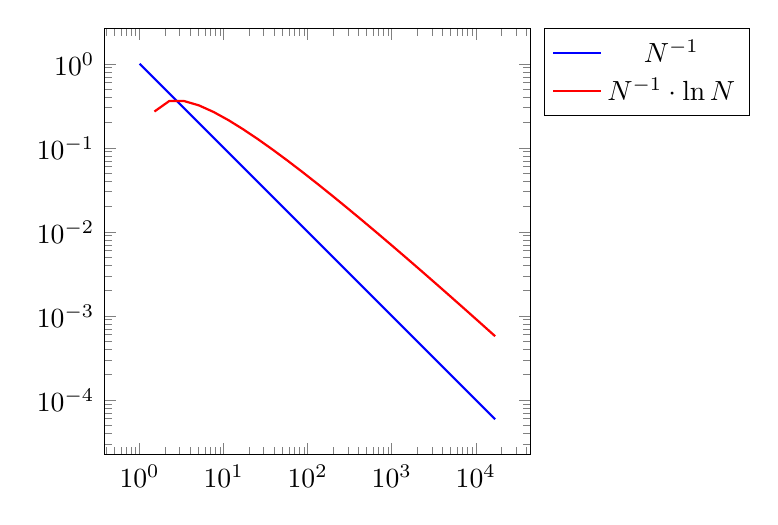
\begin{tikzpicture}
    \begin{loglogaxis}[width=7cm, height=7cm, legend pos = outer north east]
      \addplot [color=blue, thick, domain= 1:17000, variable=\x ]plot ({\x}, {1/\x}); 
      \addplot [color=red, thick, domain= 1:17000, variable=\x ]plot ({\x}, {1/\x*ln(\x)}); 
      \legend{$N^{-1}$, $N^{-1}\cdot \ln N$};
    \end{loglogaxis}
  \end{tikzpicture}
  \caption{$N^{-1}$ vs. $N^{-1} \cdot \ln N$}
  \label{fig:log}
\end{figure}



Trotzdem verdirbt der $\log$-Faktor die Konvergenzordung, speziell bei Methoden höherer Ordnung. Daher modifizieren wir die Gitter. Dabei belassen wir den Übergangspunkt $\tau$ und das Verhalten außerhalb der Grenzschicht, verändern aber das Gitter auf $[0, \tau]$. Dies wird generiert mit der Funktion $\tilde\phi$. Für diese fordern wir nur
\begin{enumerate}
\item $\tilde \phi (0) = 0$, 
\item $\tilde \phi (q) = \ln N$, 
\item $\tilde \phi$ ist monoton wachsend;
\end{enumerate}
dann erhalten wir ein \markdef{Shishkin-Typ-Gitter} oder \markdef{S-Typ-Gitter}. 
Zu dieser führen wir die charakterisierende Funktion
\begin{align*}
  \psi(t) = e^{- \tilde \phi (t)}, 
\end{align*}
die monoton fallend ist. 
\begin{folgerung}\label{6-13}
  Für $\tau = \sigma \frac \epsilon \beta \ln N$ mit $\sigma \geq 2$ gilt auf einem S-Typ-Gitter mit
  \begin{align*}
    \max_{t \in [0, q]} \tilde \phi'(t) \leq \kappa N,
  \end{align*}
  dass
  \begin{align*}
    \nnorm{u - u^{I}}_{L_{\infty}} \leq C ( h + N^{-1} \max \norm{\psi'})^{2}  
  \end{align*}
  mit
  \begin{align*}
    \max \norm{\psi'} =   \max_{t \in [0, q]} \norm{\psi'(t)} 
  \end{align*}
  und
  \begin{align*}
    \nnorm{u - u^{I}}_{L_{\infty}[\tau, 1]} \leq C \cdot N^{-2}
  \end{align*}
  und $h = \max_{i = 1, \dots, q N} h_{i} \leq C_{\epsilon}$.  
\end{folgerung}
\begin{beweis}
  Auf $[\tau, 1]$ siehe Beweis der Folgerung \ref{6-12}. 
  \begin{align*}
    \psi(t_{i}) = e^{-\tilde \phi(t_{i})} &= e^{-(\tilde \phi(t_{i}) - \tilde \phi (t))} e^{-\tilde \phi(t)}\\
    &= e^{-(\tilde \phi(t_{i}) - \tilde \phi (t))} \psi(t)\\
    &\geq e^{-N^{-1} \max \tilde\phi'(t)} \psi(t)\\
    &\geq e^{-k} \psi(t)
  \end{align*}
  für alle $t \in [t_{i-1}, t_{i}]$. Außerdem ist
  \begin{align*}
    x &= \frac{\sigma\epsilon}{\beta} \tilde \phi (t) = - \frac{\sigma\epsilon}{\beta} \ln \psi(t)\\
    \implies  \quad& \psi(t) = e^{- \frac{\beta x}{\sigma\epsilon}}\\
    \implies  \quad& \psi(t_{i}) \geq e^{-\kappa} e^{- \frac{\beta x}{\sigma\epsilon}}
  \end{align*}
  für $x \in [x_{i-1}, x_{i}]$ und
  \begin{align*}
    \tilde\phi'(t) = (- \ln  \psi(t))' = - \frac{\psi'(t)}{\psi (t)}. 
  \end{align*}
  Nach diesen Vorüberlegungen folgt für $h_{i}$:
  \begin{align*}
    h_{i} &= x_{i} - x_{i-1} = \frac{\sigma\epsilon}{\beta} \( \tilde \phi (t_{i}) - \tilde \phi (t_{i-1})\) = \frac{\sigma\epsilon}\beta \int_{t_{i-1}}^{t_{i}} \tilde \phi ' (t) dt\\
    &\leq \frac {\sigma\epsilon}\beta N^{-1}\max_{t \in [t_{i-1}, t_{i}]} \tilde \phi'(t)\\
    \implies \quad & h_{i} \leq C \epsilon, \quad i = 1, \dots, qN\\
    &\leq \frac{\sigma\epsilon}\beta N^{-1} \frac{\max_{t\in [t_{i-1}, t_{i}]} \norm{\psi'(t)}}{\psi (t_{i})}\\
    & \leq \frac {\sigma\epsilon}{\beta} N^{-1} e^{\kappa} e^{\frac {\beta x}{\sigma\epsilon}} \max\norm{\psi'} = C \epsilon N^{-1} \max\norm{\psi'} e^{\frac{\beta x}{\sigma\epsilon}}. 
  \end{align*}
  Nun fügen wir zusammen: 
  \begin{align*}
    \theta_{i} &= \int_{x_{i-1}}^{x_{i}} \(1 + \epsilon^{-1} e^{ - \frac{\beta x}{2 \epsilon}}\) dx\\
    & \leq h_{i} + \epsilon^{-1} h_{i} e^{- \frac{\beta x_{i-1}}{ 2 \epsilon}}\\
    & \leq h_{i} + C N^{-1}\max \norm{\psi'} e^{\frac{\beta x}{ \sigma\epsilon}} e^{- \frac{\beta x_{i-1}}{ 2 \epsilon}}\\
    & \leq h_{i} + C N^{-1}\max \norm{\psi'} e^{\frac{\beta x_{i-1}}{ \sigma\epsilon}}e^{\frac{\beta s\cdot h_{i}}{ \sigma\epsilon}}e^{- \frac{\beta x_{i-1}}{ 2 \epsilon}}\\
    & \leq h_{i} + C N^{-1}\max \norm{\psi'} e^{\frac{\beta x_{i-1}}{ \epsilon} \cdot\(\frac 1 \sigma - \frac 1 2\)}e^{\frac{\beta \cdot s\cdot C}{ \sigma}}\\
    % & \leq h_{i} + C N^{-1}\max \norm{\psi'} e^{\frac{\beta}{\epsilon} \(\frac {x_{i}} \sigma - \frac {x_{i-1}} 2\)}\\
    % & \leq h_{i} + C N^{-1}\max \norm{\psi'} e^{\frac{\beta h_{i}}{\sigma\epsilon} } e^{\frac{\beta x_{i-1}}{\epsilon} (\frac 1 \sigma - \frac 12)}\\
    % & \leq h_{i} + C N^{-1}\max \norm{\psi'} e^{\frac{\beta x_{i-1}}{\epsilon} (\frac {2 -  \sigma} {2 \sigma})}\\
    & \leq h + C N^{-1}\max \norm{\psi'}. 
  \end{align*}
  mit $s \in (0, 1)$, da $\sigma\geq 2$.
\end{beweis}
\paragraph{S-Typ Gitter aus der Literatur}
\label{sec:s-typ-gitter}
\begin{enumerate}
\item Standart Shishkin-Gitter
  \begin{align*}
    \tilde \phi (t) &= \frac t q \ln N \implies \psi(t) =  e^{- \frac t q \ln N}\\
    \max \norm{\psi'} &\leq \frac{\ln N} q, \\
    h &\leq \frac{\sigma\epsilon} \beta N^{-1} \frac{\ln N} q \leq C N^{-1}\\
    \implies \quad h + \max \norm{\psi'} &\leq C \cdot N^{-1} \ln N. 
  \end{align*}
  (Folgerung \ref{6-12}). 
\item Bakhvalov -S-Gitter
  Invertiere $e^{- \frac{\beta x}{\sigma\epsilon}}$ auf $[0, \tau]$ und Shishkin-Definitionen von $\tau$ und gleichmäßiges Gitter auf $[\tau, 1]$.
  \begin{align*}
    \tilde \phi (t) &= - \ln ( 1- (1 - N^{-1}) \frac t q)\\
    \implies \quad  \psi(t) &= 1 -(1 - N^{-1})\frac t q\\
    \implies \max \norm {\psi'} &= \frac 1 q (1 - N^{-1}) \leq \frac 1q\\
    \max \norm{\tilde \phi'(t)}&\leq \frac 1 q N \implies h \leq \frac{\sigma\epsilon}\beta \frac{N^{-1} N} q \leq C \epsilon\\
    \implies h +  N^{-1}\max \norm{\psi'} &\leq C (\epsilon + N^{-1})
  \end{align*}
  ist optimal für $\epsilon \leq CN^{-1}$. 
\item Polynomiales Gitter
  \begin{align*}
    \tilde \phi (t) = \(\frac t q\)^{m} \ln N, \quad m \geq 1, \quad \implies \psi (t) = N^{- \frac(t q)^{m}} \\
    \dots \implies \quad \max \norm{\psi'} \leq & C (\ln N)^{\frac 1m}, \quad h \leq m N^{-1}\\
  \end{align*}
  Für $m \geq 1$ ist das besser als das Shishkin-Gitter, aber immer noch schlechter als das Bakhvalov-Shiskin-Gitter. 
\end{enumerate}
Für die Fehleranalysis bei FEM benötigen wir Interpolationsfehlerschranken in der Energienorm $\nnnorm \cdot _{\epsilon}$.
\begin{satz}\label{thm:6-14}
  Es gilt für die lineare Interpolierende $v^{I}$ mit
  \begin{align*}
    \norm{v''} &\leq C (1 + \epsilon^{-2} e^{- \frac {\beta x}\epsilon}\\
    \nnnorm{v^{I} - v}_{\epsilon} &\leq C (\nnorm{v^{I} - v}_{L_{\infty}})^{\frac 12}. 
  \end{align*}
\end{satz}
\begin{beweis}
  \begin{align*}
    \nnorm{v^I - v}_{L_{2}} &\leq \nnorm{v^I - v}_{L_{\infty}}\\
    \epsilon\nnorm{(v^I - v)'}_{L_{2}} ^{2} &= \epsilon \int_{0}^{1} ((v^{I} - v) (x))^{2} dx = - \epsilon \int_{0}^{1} v''(x)(v - v^{I}) (x) dx\\
    &\leq \nnorm{v - v^{I}}_{L_{\infty}} \epsilon \int_{0}^{1} \norm{v''(x)} dx\\
    &\leq C\nnorm{v - v^{I}}_{L_{\infty}} 
  \end{align*}
\end{beweis}
\begin{lemma*} Inverse Ungleichungen
  Sei  $w$ eine lineare Funktion auf $[x_{i-1}, x_{i}]$. Dann gilt
  \begin{align*}
    \nnorm{w'}_{L_{2}(x_{i-1}, x_{i})} \leq 2 \frac{\sqrt 3}{h_{i}} \nnorm{w}_{L_{2}(x_{i-1}, x_{i})}. 
  \end{align*}
\end{lemma*}
\begin{beweis}O.B.d.A sei $x_{0} = 0, x_{1} = h$. 
  \begin{align*} 
    w &= w_{0} + \frac{w_{1} - w_{0}} h x\\
    w' &=\frac{w_{1} - w_{0}} h x\\
    \nnorm{w'}_{L_{2}}^{2} &=\frac{(w_{1} - w_{0})^{2}} h \\
    \nnorm{w}_{L_{2}}^{2} &= \int_{0}^{h} (w_{0} + \frac{(w_{1} - w_{0})} hx)^{2} dx \\
    &= \int_{w_{0}}^{w_{1}} t^{2} \frac{ h }{(w_{1} - w_{0})} dt \\
    &= \frac h 3 \frac{w_{1}^{3} - w_{0}^{3}}{w_{1} - w_{0}} = \frac h 3 (w_{1}^{2} + w_{1}w_{0} + w_{0}^{2})
  \end{align*}
  mit der Substitution $t = w + \frac {w_{1} - w_{0}} h x$. Weiter
  \begin{align*}
    \frac {\nnorm {w'}_{L_{2}}^{2}}{\nnorm {w'}_{L_{2}}^{2}} &= \frac 3 {h^{2}} \frac{(w_{1} - w_{0})^{2}} {w_{1}^{2} + w_{1}w_{0} w_{0}^{2}} \\
    &= \frac 3 {h^{2}} \frac {(w_{1} - w_{0})^{2}}{\frac 34 (w_{1} + w_{0})^{2} + \frac 14 (w_{1} - w_{0})^{2}} \leq \frac {12}{h^{2}}. 
  \end{align*}
  Die inverse Ungleichung
  \begin{align*}
    \nnorm{w'}_{L_{2}(x_{i-1}, x_{i})} &\leq  C h_{i}^{-1} \nnorm{w}_{L_{2}(x_{i-1}, x_{i})}\\
    \nnorm{\partial^{l} w}_{L_{p}(x_{i-1}, x_{i})} &\leq  C h_{i}^{m - l + (\frac 1 p - \frac 1 q)} \nnorm{\partial^{m} w}_{L_{q}(x_{i-1}, x_{i})}\\
  \end{align*}
  gilt für jedes Polynom $w \in \Pi_{k}$. Der Beweis läuft im Allgemeinen über
  \begin{itemize}
  \item Transformation auf $[0, 1]$, 
  \item Äquivalenz von Normen auf endlich-dimensionalen Räumen, 
  \item Rücktransformation auf $[x_{i-1}, x_{i}]$. 
  \end{itemize}
\end{beweis}
% \datum{03. Dezember und Do Woche davor fiel aus}
% \datum{04. Dezember 2015}
\begin{satz}\label{thm:6-15}
  Auf einem S-Typ-Gitter mit $\sigma \geq 2$ und einer charakterisierenden Funktion $\psi$ mit
  \begin{align*}
    N^{-1} \max \norm{\psi'}(\ln N)^{\frac 12} \leq C
  \end{align*}
  gilt für lineare Finite Elemente
  \begin{align*}
    \nnnorm{u-u_{h}}_{\epsilon} \leq C (h + N^{-1} \max \norm{\psi'}). 
  \end{align*}
\end{satz}
\begin{beweis}
  Sei $\eta  = u^{I} - u$ und $\chi = u^{I} - u_{h}$. Mit Satz \ref{thm:6-14} und der Folgerung \ref{6-13} erhalten wir
  \begin{align*}
    \nnnorm{\eta}_{\epsilon} \leq C (h + N^{-1} \max \norm{\psi'}).
  \end{align*}
  Für $\chi$ nutzen wir die Koerzivität und die Galerkin-Orthogonalität:
  \begin{align*}
    \nnnorm{\chi}^{2}_{\epsilon} \leq a(\chi, \chi) = a (\eta, \chi) = \epsilon (\eta', \chi') + (b \eta, \chi') + (c \eta, \chi)
  \end{align*}
  Mit Cauchy-Schwarz erhalten wir für den Diffusions- ($\epsilon (\eta', \chi')$) und den Reaktionsterm ($(c \eta, \chi)$) sowie Hölder für den Konvektionsterm ($(b \eta, \chi')$):
  \begin{align*}
    \nnnorm{\chi}^{2}_{\epsilon} \leq C \nnnorm{\eta}_{\epsilon} \nnnorm{\chi}_{\epsilon}+ \(\nnorm{\eta}_{L_{\infty}(0, \tau)}\nnorm{\chi'}_{L_{1}(0, \tau)} + \nnorm{\eta}_{L_{2}(\tau, 1)}\nnorm{\chi'}_{L_{2}( \tau, 1)} \). 
  \end{align*}
  Auf $[0, \tau]$ nutzen wir die Kleinheit des Gebietes beim Übergang von $L_{1}$ nach $L_{2}$. Auf $[\tau, 1]$ hingegen benötigen wir eine inverse Ungleichung
  \begin{align*}
    \nnorm{\chi'}_{L_{2}( \tau, 1)} &\leq C H^{-1} \nnorm{\chi}_{L_{2}( \tau, 1)} \leq C N \nnorm{\chi}_{L_{2}( 0, 1)}\\
    \implies \nnnorm{\chi}^{2}_{\epsilon} &\leq C \nnnorm{\eta}_{\epsilon} \nnnorm{\chi}_{\epsilon}+ C\cdot\(\nnorm{\eta}_{L_{\infty}(0, \tau)} (\epsilon \ln N)^{\frac 12}\nnorm{\chi'}_{L_{2}(0, \tau)} + \nnorm{\eta}_{L_{2}(\tau, 1)}N\nnorm{\chi}_{L_{2}(\tau, 1)} \) \\
    &\leq C \( h + N^{-1} \max \norm{\psi'} + (h + N^{-1} \max \norm{\psi'})^{2} (\ln N)^{\frac 12} + \frac{N^{-2}}{N}\) \nnnorm{\chi}_{\epsilon}. 
  \end{align*}
  Zeige nun: das ist beschränkt! Nutze $h\cdot \epsilon (\ln N)^{\frac 12} \leq C \epsilon^{ \frac 12} \leq C$ und die Voraussetzung der Beschränktheit an die Funktion $\psi$. Also
  \begin{align*}
    \nnnorm{\chi}_{\epsilon} \leq C (h + N^{-1} \max \norm{\psi'}). 
  \end{align*}
\end{beweis}
Die Galerkin FEM ist somit gleichmäßig konvergent mit Ordnung fast $1$ (wegen $\max \norm {\psi'}$), wie der Interpolationsfehler
\begin{align*}
  \nnnorm {u - u_{h}}_{\epsilon} \leq C \inf_{v_{h} \in V_{h}} \nnnorm{u - v_{h}}_{\epsilon} \leq C \nnnorm{u - u^{I}}_{\epsilon}. 
\end{align*}
mit Cea. Aber die numerische Lösung ist sogar bezüglich der Interpolierenden besser: 
\begin{satz}\label{thm:6-16}
  Auf einem S-Typ-Gitter mit $\sigma \geq \frac 52$ gilt für die Lösung $u_{h}$ der linearen Galerkin-FEM und für $u^{I}$, die lineare Interpolierende
  \begin{align*}
    \nnnorm{u^{I} - u_{h}}_{\epsilon} \leq C (h^{2} (\ln N)^{\frac 12} + (N^{-1} \max \norm{\psi'}) ^{2}). 
  \end{align*}
\end{satz}
\begin{beweis}
  Sei erneut $\eta = u-u^{I}$ und $\chi = u^{I} - u_{h}$. Dann folgt
  \begin{align*}
    \nnnorm{\chi}_{\epsilon}^{2} \leq a(\eta, \chi) = \epsilon(\eta', \chi') - (b \eta', \chi) + (c \eta, \chi). 
  \end{align*}
  Für den Diffusionsterm erhalten wir mit partieller Integration
  \begin{align*}
    (\eta', \chi')_{I_{i}} = \eta \chi'|_{x_{i-1}}^{x_{i}} - \int_{x_{i-1}}^{x_{i}} \eta\chi'' dx = 0
  \end{align*}
  Es ist $\eta(x_{j}) = 0$ für alle $j$ und $\chi'' = 0$, da $\chi$ linear ist. Für den Reaktionsterm liefert Cauchy-Schwarz
  \begin{align*}
    \norm{(c \eta, \chi)} \leq C \nnorm{\eta}_{L_{2}} \nnorm{\chi}_{L_{2}} \leq C(h + N^{-1} \max \norm {\psi'})^{2} \nnnorm{\chi}_{\epsilon}. 
  \end{align*}
  Bleibt nur noch der Konvektionsterm (wie üblich ist das der schwierigste Term). Dafür nutzen wir die Zerlegung (Satz \ref{thm:5-2})
  \begin{align*}
    u = S+E
  \end{align*}
  und nehmen $b$ als konstant an. Für variables $b$ erhalten wir nur zusätzliche Terme, die sich wie der Reaktionsterm behandeln lassen. Dann folgt
  \begin{align*}
    (\eta', \chi) &=- \int_{0}^{\tau} (E^{I} - E)\cdot\chi' - \int_{0}^{\tau} (S^{I} - S)\cdot \chi' - \int_{\tau}^{1} (E^{I} - E)\chi' + \int_{\tau}^{1}(S^{I} - S)' \chi\\
    &= i + ii + iii + iv. 
  \end{align*}
  \begin{enumerate}
  \item zu i: Standard-Interpolationsfehlerabschätzung liefert
    \begin{align*}
      \nnorm{E^{I} - E}_{L_{2} (x_{i-1}, x_{i})} \leq C h_{i}^{2} \nnorm{E''}_{L_{2}(x_{i-1}, x_{i})}
    \end{align*}
    und damit
    \begin{align*}
      \norm { \int_{0}^{\tau} (E^{I} - E)\cdot\chi'} &\leq  \nnorm{E^{I} - E}_{L_{2} (0, \tau)} \cdot \nnorm{\chi'}_{L_{2} (0, \tau)}\\
      & \leq C \( \sum_{i =1}^{qN} h_{i}^{4}  \int_{x_{i-1}}^{x_{i}} \epsilon^{-4} e^{-2 \beta \frac x \epsilon} dx \)^{\frac 12} \nnorm{\chi'}_{L_{2} (0, \tau)}\\
      & \leq C \( \sum_{i =1}^{qN} \int_{x_{i-1}}^{x_{i}} \epsilon^{4}(N^{-1} \max \norm{\psi'})^{4} e^{4 \frac{\beta  x} {\sigma \epsilon}} \epsilon^{-4} e^{-2 \beta \frac x \epsilon} dx \)^{\frac 12} \nnorm{\chi'}_{L_{2} (0, \tau)}\\
      & \leq C (N^{-1} \max \norm{\psi'})^{2} \( \int_{0}^{\tau} e^{(\frac 4 \sigma - 2)  \frac{\beta  x} { \epsilon}} dx \)^{\frac 12} \nnorm{\chi'}_{L_{2} (0, \tau)}\\
    \end{align*}
    wobei nach Voraussetzung $\frac 4 \sigma - 2 <0$ ist, und es ist $\sigma > 2$. Also folgt weiter
    \begin{align*}
      & \leq C (N^{-1} \max \norm{\psi'})^{2} \(\frac{\epsilon}{\beta \norm{\frac 4 \sigma - 2}}\)^{\frac 12} \nnorm{\chi'}_{L_{2} (0, \tau)}\\
      & \leq C (N^{-1}\max \norm{\psi'})^{2} \nnnorm{\chi'}_{\epsilon}. 
    \end{align*}
  \item zu ii:
    \begin{align*}
      \norm{\int_{0}^{\tau} (S^{I} - S) \chi'} &\leq C \( \sum_{i =1}^{qN} h_{i}^{4}  \nnorm{S''}^{2}_{L_{2}(x_{i-1}, x_{i})} \)^{\frac 12} \nnorm{\chi'}_{L_{2} (0, \tau)}\\
      &\leq C h^{2} \underbrace{\nnorm{S''}^{2}_{L_{2}(0, \tau)}}_{C \cdot meas (0, \tau)^{\frac 12}} \nnorm{\chi'}_{L_{2} (0, \tau)}\\
      &\leq C h^{2} (\epsilon \ln N)^{\frac 1 2}\nnorm{\chi'}_{L_{2} (0, \tau)}\\
      &\leq C h^{2} (\ln N)^{\frac 1 2}\nnorm{\chi'}_{\epsilon}. 
    \end{align*}
  \item zu iii: Wir zerlegen $[\tau, 1]$ in $[\tau, \tau + H]$ und $[\tau + H, 1]$. Dann gilt
    \begin{align*}
      \nnorm{E^{I} - E}^{2}_{L_{2} (\tau, \tau + H)} \leq H \max_{(\tau, \tau + H)} \set{\norm{E^{I}}, \norm{E}}^{2} \leq 2 H \nnorm{E}^{2}_{L_{\infty}(\tau, \tau + H)} = 2 H e^{ - \frac{2 \beta \tau}{\epsilon}} \leq C N^{-1} N^{-2 \sigma} \leq C N^{-6}
    \end{align*}
    $E$ ist monoton fallend, und $\tau = \frac {\sigma\epsilon \ln N} \beta$ und $\sigma \geq \frac 5 2$. Also folgt mit einer inversen Ungleichung
    \begin{align*}
      \norm{\int_{\tau}^{\tau + H} (E^{I} - E) \chi'} &\leq C \nnorm{E^{I} - E}_{L_{2} (\tau, \tau + H)} H^{-1} \nnorm{\chi}_{L_{2}(\tau, \tau +H)}\\
      &= C N^{-3} N \nnorm{\chi}_{\epsilon} \leq  CN^{-2}\nnorm{\chi}_{\epsilon}. 
    \end{align*}
    Im Rest gilt
    \begin{align*}
      \nnorm{E^{I} - E}^{2}_{L_{2} (\tau + H, 1)} &= \sum_{i = qN + 2}^{N}   \nnorm{E^{I} - E}^{2}_{L_{2} (x_{i-1}, x_{i})} \\
      &\leq \sum_{i = qN + 2}^{N} H \nnorm{E^{I} - E}^{2}_{L_{\infty} (x_{i-1}, x_{i})} \\
      &\leq 2 \sum_{i = qN + 2}^{N} H \nnorm{E}^{2}_{L_{\infty} (x_{i-1}, x_{i})} \\
      &\leq C \sum_{i = qN + 2}^{N} H e^{ - 2 \frac{\beta x_{i-1}}{\epsilon}}\\
      &= C \sum_{i = qN + 2}^{ N} \int_{x_{i-2}}^{x_{i-1}} e^{ - 2 \frac{\beta x_{i-1}}{\epsilon}} dx\\
      &= C \sum_{i = qN + 2}^{ N} \int_{x_{i-2}}^{x_{i-1}} e^{ - 2 \frac{\beta x}{\epsilon}} dx\\
      &= C \int_{\tau}^{x_{N-1}}  e^{ - 2 \frac{\beta x}{\epsilon}} dx\\
      &\leq C \epsilon N^{- 2\sigma}\\
      &\leq C \epsilon N^{- 5}\\
      \implies \quad \norm{\int_{\tau + H}^{1} (E- E^{I}) \chi'} &\leq C \nnorm{E - E^{I}}_{L_{2}(\tau + H, 1)}  \nnorm{\chi'}_{L_{2}(\tau + H, 1)} \\
      &\leq C \epsilon^{ \frac 12} N^{ - \frac 5 2} \nnorm{\chi'}_{L_{2}(0, 1)}\\
      &\leq C N^{ - \frac 5 2} \nnnorm{\chi}_{\epsilon}\\
      \implies \quad \norm{\int_{\tau}^{1} (E- E^{I}) \chi'} &\leq C N^{-2} \nnnorm{\chi}_{\epsilon}
    \end{align*}
    (Shift im Integral und wir landen wieder bei der $L_{2}$-Norm!!)
  \item zu iv: Der friedfertigste Term ist der schwierigste: Hier nutzen wir eine der Lin-Identitäten (Lin: chinesischer Mathematiker): Mit
    \begin{align*}
      E_{i}(x) &= \frac 12 \( (x - x_{i- \frac 12})^{2} - \( \frac {h_{i}} 2\)^{2} \)\\
      &= \frac 12 (x - x_{i-1}) \cdot (x - x_{i})
    \end{align*}
    gilt für ein $v \in W^{3, \infty}(x_{i-1}, x_{i})$:
    \begin{align*}
      \int_{x_{i-1}}^{x_{i}} (v - v^{I})' \chi &= \frac 16 \int_{x_{i-1}}^{x_{i}} v''' (E_{i}^{2})' \chi' - \frac 13 \(\frac{h_{i}} 2\)^{2} \int_{x_{i-1}}^{x_{i}} v''' \chi + \frac 1 3 \( \frac {h_{i}} 2\)^{2} v'' \chi|_{x_{i-1}}^{x_{i}}.
    \end{align*}
    Wir erhalten daher
    \begin{align*}
      \int_{\tau}^{1} (S^{I} - S)' \chi &= frac 1 6 \int_{\tau}^{1} S''' (E^{2})' \chi' - \frac{H^{2}}{12} \int_{\tau}^{1} S''' \chi - \frac {H^{2}}{ 12} (S''\chi)(\tau).
    \end{align*}
    Mit $\norm{S^{(k)}\leq C}, k = 2, 3$ folgt mit der inversen Ungleichung
    \begin{align*}
      \norm{\int_{\tau}^{1} (S^{I} - S)' \chi} &\leq C \( H^{3} \nnorm{\chi'}_{L_{1}(\tau, 1)} + H^{2} \nnorm{\chi}_{L_{1}(\tau, 1)} + H^{2} \norm{\chi(\tau)} \)\\
      &\leq C \( H^{2} \nnorm{\chi}_{L_{2}(\tau, 1)} + H^{2} \norm{\chi(\tau)}\).  
    \end{align*}
    Mit
    \begin{align*}
      \norm{\chi(\tau)} &=\norm{ \int_{0}^{\tau} \chi'(\tau) dt} \leq \tau^{\frac 12}  \nnorm{\chi'}_{L_{2}(0, \tau)} \leq C (\ln N)^{\frac 12} \nnnorm \chi_{\epsilon}\\
      \implies \quad \norm{ \int_{\tau}^{1} (S^{I} - S)' \chi} &\leq  C N^{-2} (\ln N)^{\frac 12}  \nnnorm \chi_{\epsilon}
    \end{align*}
  \end{enumerate}
\end{beweis}
% \datum{10. Dezember 2015}

Erstaunlicherweise ist nicht der Grenzschichtanteil, sondern der glatte Anteil $S$ in der Abschätzung der problematische. Hier haben wir dazu die Integralidentität von Lin benutzt. Eine Eigenschaft wie in Satz \ref{thm:6-16} heißt \markdef{supercloseness}, hier bezüglich der Interpolierenden in der Energienorm (näher an der Interpolierenden als an der echten Lösung). Wie lässt sich das praktisch nutzen?

\paragraph{Postprocessing (Nachbearbeitung)}
\label{sec:postpr-nachb}

Die Idee des Postprocessings ist es, mithilfe einer preiswerten Methode aus der bereits berechneten numerischen Lösung eine neue numerische Lösung zu gewinnen. Es gibt viele Möglichkeiten, hier besprechen wir einen Ansatz, der die vorhandene Lösung in einen Polynomraum höherer Ordnung auf einenm gröberen Gitter interpolieren (nach \cite{ST_SINUM}). Zu dem vorhandenen Gitter $T_{N}$ konstruieren wir uns ein Makrogitter $M_{N}$, indem je zwei Gitterzellen zu einer Makrozelle zusammengefasst werden. 
\begin{figure}[ht!]
  \centering
  \begin{tikzpicture}
    
    \newcommand*{\xMin}{0}%
    \newcommand*{\xMax}{6}%
    \newcommand*{\yMin}{0}%
    \newcommand*{\yMax}{6}%
    \def\Ncoarse {6};
    \def\Nfine {10};
    \def\lambday  {0.3};
    \def\lambdax {0.3};
    \def\h { (\xMax -\lambdax)/\Ncoarse};
    
    \def\picscale {0.00125};
    \pgfmathsetmacro\newvalue{\lambdax + \h * \picscale * \Nfine * \Nfine * \Nfine};
    \pgfmathsetmacro\hfine{(\newvalue/\Nfine)};

    \begin{scope}[scale = 2]
      \foreach \i in {0, 2, 4, 6, 8} {
        \pgfmathsetmacro\xcoord{\hfine*\i};
        \draw [very thin,red] (\xcoord, \yMin-0.1) -- (\xcoord, \yMin+0.1);% node [below] at (\xcoord*10,\yMin) {\hfine};
        \pgfmathsetmacro\xcoord{\hfine*(\i+1)};
        \draw [very thin,gray] (\xcoord, \yMin-0.1) -- (\xcoord, \yMin+0.1);% node [below] at (\xcoord,\yMin) {$\i$};
      }
      % \foreach \i in {0,...,\Nfine} {
      % \pgfmathsetmacro\ycoord{(\lambday + \h*\i*\i*\i) * \picscale};
      \draw [very thin,gray] (\xMin,0) -- (\xMax,0);% node [left] at (\xMin,\ycoord) {$\i$};
      % }

      \foreach \i in {0, 2, 4} {
        \pgfmathsetmacro\xcoord{\newvalue * (\i * 0.16666) + \xMax * (\Ncoarse - \i) * 0.16666};
        \draw [very thin,red] (\xcoord, \yMin-0.1) -- (\xcoord, \yMin+0.1);% node [below] at (\xcoord,\yMin) {$\i$};
        \pgfmathsetmacro\xcoord{\newvalue * ((\i+1) * 0.1666) + \xMax * (\Ncoarse - (\i+1)) * 0.1666};
        \draw [very thin,gray] (\xcoord, \yMin-0.1) -- (\xcoord, \yMin+0.1);% node [below] at (\xcoord,\yMin) {$\i$};
      }


      \draw[thick,red] (\newvalue, \yMin -0.1) -- (\newvalue, \yMin+0.1) node [below] at (\newvalue, \yMin) {$\tau \in M$};

      \node[below] at (\newvalue - .7, \yMin -0.1) {$h$};
      \node[below] at (\newvalue + 1.1, \yMin -0.1) {$H$};
      % \draw[thick,black] (\xMin, \newvalue) -- (\xMax, \newvalue) node [left] at (\xMin, \newvalue) {$\lambda_{y}$};
      \node [below left] at (0, 0) {$0$};
      \node [below right] at (\xMax, 0) {$1$};
      % \node [left] at (0, \yMax) {$1$};
    \end{scope}
  \end{tikzpicture}

  \caption{Makro-Mikro-Gitter, $M_{N}$ rot, $T_{N}$ schwarz}
  \label{fig:macro-micro-grid}
\end{figure}

Da auf einem S-Typ-Gitter die Schrittweiten $h$ und $H$ unterschiedliche Größenordnungen bezüglich $\epsilon$ haben, sollte kein Makroelement aus einer kleinen und einer großen Zelle bestehen (also sollte die Grenze $\tau$ im Makrogitter auch Grenze sein). Sei daher $qN$ und $(1-q)N$ gerade, zum Beispiel $q = \frac 12$ und $N \mod 4 = 0$. Im Allgemeinen wird $M_{N} \neq T_{\frac N 2}$ sein, da $\tau$ und $\phi$ nicht dieselben sind! Wir definieren nun den Projektor
\begin{align*}
  P: \, C[0, 1] \to W_{h} \coloneqq \set{w \in C[0, 1]: \, w|_{(x_{i-1}, x_{i+1})} \in \Pi, \, i = 1, 3, 5, \dots, N-1}
\end{align*}
lokal als quadratische Interpolierende, das heißt
\begin{align*}
  Pv(x_{i-1}) &= v(x_{i-1}),\\
  Pv(x_{i}) &= v(x_{i}),\\
  Pv(x_{i+1}) &= v(x_{i+1}),\\
  Pv|_{(x_{i-1}, x_{i+1})} &\in \Pi_{2}.
\end{align*}
Im Allgemeinen besteht ein Makroelement im Grenzschichtbereich nicht aus zwei gleich großen Zellen. Die Hoffnung ist, dass die beiden Zellen nicht allzu unterschiedlich sind. Dazu muss zur Abschätzung der Interpolation mit $P$ eine Annahme an die Gitterweiten im Grenzschichtbereich gestellt werden. Genauer existiere ein $p\geq 1$ mit
\begin{align*}
  \frac{\max \set{h_{i}, h_{i+1}}}{\min \set{h_{i}, h_{i+1}}}\leq p
\end{align*}
für $i = 1, 3, \dots, \frac {qN} 2 - 1$. Erfüllen unsere Gitter das? Für die bislang betrachteten S-Typ-Gitter gilt Tablle \ref{tab:gitter_u_h}. 
\begin{table}[h!]
  \centering
  \begin{tabular}[h!]{l l}
    Shishkin-Gitter: & $h_{i} = h_{i+1}$, also $p = 1$\\
    Bakhvalov-Gitter: & $h_{i} < h_{i+1}$ und $\frac{h_{i+1}}{h_{i}} \leq \frac{h_{qN}}{h_{qN-1}} \leq \frac{\ln 3}{\ln \frac 53} \eqqcolon p$\\
    polynomiale Gitter: & $m \geq 1$, also $h_{i}< h_{i+1}$, $\frac{h_{i+1}}{h_{i}} \leq \frac{h_{2}}{h_{1}} = 2^{m} -1 \eqqcolon p$
  \end{tabular}
  \caption{Gitter und $p$}
  \label{tab:gitter_u_h}
\end{table}
\begin{lemma}\label{lem:6-17}
  Es sei $T_{N}$ ein S-Typ-Gitter mit $p\geq 1$. Dann gilt
  \begin{align*}
    \nnorm{Pw}_{L_{\infty}(x_{i-1}, x_{i+1})} \leq C \cdot\nnorm{w}_{L_{\infty}(x_{i-1}, x_{i+1})}
  \end{align*}
  und
  \begin{align*}
    \nnorm{(Pw)'}_{L_{\infty}(x_{i-1}, x_{i+1})} \leq C \cdot\nnorm{w'}_{L_{\infty}(x_{i-1}, x_{i+1})}. 
  \end{align*}
  Das sind Stabilitätseigenschaften des Operators bezüglich $\nnorm \cdot_{L_{\infty}}$ und $\nnorm \cdot_{W^{1, \infty}}$.
\end{lemma}
\begin{beweis}
  Wir haben die Lagrange-Basisfunktionen $L_{i-1}, L_{i}, L_{i+1}$ zu $x_{i-1}, x_{i}, x_{i+1}$ und 
  \begin{align*}
    \nnorm{Pw}_{L_{\infty}(x_{i-1}, x_{i+1})} &= \nnorm{L_{i-1}(x)w_{i-1} + L_{i}(x)w_{i} + L_{i+1}(x)w_{i+1}}_{L_{\infty}(x_{i-1}, x_{i+1})}\\
    &\leq 3\cdot \nnorm{w}_{L_{\infty}(x_{i-1}, x_{i+1})} \cdot \max_{j}\nnorm{L_{j}(x)}_{L_{\infty}(x_{i-1}, x_{i+1})}. 
  \end{align*}
  Nun gilt
  \begin{align*}
    L_{i-1}(x) &= \frac{(x-x_{i})(x-x_{i+1})}{(x_{i-1}-x_{i})(x_{i-1}-x_{i+1})}\\
    \implies   \norm {L_{i-1}(x)} &\leq \max\set{1, \frac{h_{i+1}^{2}}{4\cdot h_{i}(h_{i} + h_{i+1})}}\\
    &\leq \max\set{1, \frac p 4}\\
    L_{i}(x) &= .\frac{(x-x_{i-1})(x-x_{i+1})}{h_{i} h_{i+1}}\\
    \implies   \norm {L_{i}(x)} &\leq \frac{(h_{i} + h_{i+1})^{2}}{4\cdot h_{i}\cdot h_{i+1}} \leq \frac {p+1} 2.  
  \end{align*}
  (Scheitelpunkt der Parabel). Es folgt
  \begin{align*}
    \nnorm{Pw}_{L_{\infty}(x_{i-1}, x_{i+1})} \leq 3 \cdot \max\set{1, \frac {p+1}2} \nnorm{w}_{L_{\infty}(x_{i-1}, x_{i+1})}. 
  \end{align*}
  Mit $L_{i-1} (x) + L_{i} (x) + L_{i+1} (x)  = 1$ folgt $(L_{i-1} (x) + L_{i} (x) + L_{i+1} (x))'  = 0$.
  \begin{align*}
    \nnorm{(Pw)'}_{L_{\infty}(x_{i-1}, x_{i+1})} &=\nnorm{L_{i-1}' (x) w_{i-1} + L_{i}' (x)w_{i} + L_{i+1}' (x)w_{i+1} }_{L_{\infty}(x_{i-1}, x_{i+1})}\\
    &= \nnorm{L_{i-1}' (x)( w_{i-1}-w_{i}) + L_{i+1}' (x)(w_{i+1}-w_{i})}_{L_{\infty}(x_{i-1}, x_{i+1})}\\
    &\leq \( h_{i}\nnorm{L_{i-1}'}_{L_{\infty}(x_{i-1}, x_{i+1})} + h_{i+1} \nnorm{L_{i+1}'}_{L_{\infty}(x_{i-1}, x_{i+1})}\) \nnorm{w}_{L_{\infty}(x_{i-1}, x_{i+1})}. 
  \end{align*}
  Da
  \begin{align*}
    \norm{h_{i} L_{i-1}'(x)} = \norm{\frac{2x - x_{i-1} - x_{i}}{h_{i} + h_{i+1}}} \leq \max\set{\frac{2h_{i+1} + h_{i}}{h_{i} + h_{i+1}}, \frac{h_{i}}{h_{i} + h_{i+1}}} \leq 1 + p
  \end{align*}
  folgt
  \begin{align*}
    \nnorm{(Pw)'}_{L_{\infty}(x_{i-1}, x_{i+1})} &\leq 2(1+p) \cdot\nnorm{w'}_{L_{\infty}(x_{i-1}, x_{i+1})}.   
  \end{align*}
\end{beweis}
Noch eine zweite Möglichkeit, den Interpolationsfehler abzuschätzen:
\begin{lemma}\label{lem:6-18}
  Es sei $T_{N}$ ein S-Typ-Gitter mit $\sigma > 2$ und $p \geq 1$. Dann gilt
  \begin{align*}
    \nnnorm{u - Pu}_{\epsilon} \leq C \( \epsilon^{\frac 12} h^{2} + (N^{-1} \max\norm {\psi'})^{2} + \epsilon N^{- \sigma +1}\). 
  \end{align*}
\end{lemma}
\begin{beweis}
  Mit der 1D-Interpolationsfehlerdarstellung folgt
  \begin{align*}
    \nnorm{v - Pv}_{L_{2}(x_{i-1}, x_{i+1})} \leq C \cdot (h_{i} + h_{i+1})^{3} \nnorm{v''}_{L_{2}(x_{i-1}, x_{i+1})}. 
  \end{align*}
  Die Lösungszerlegung von Satz \ref{thm:5-2} lautet $u = S+E$. Dann folgt
  \begin{align*}
    \nnorm{S - PS}^{2}_{L_{2}} &= \sum_{M \in M_{N}} \norm{S - PS}_{L_{2} (M)}^{2} \\
    &\leq C \sum_{M \in M_{N}} (h_{i} + h_{i-1})^{6} \norm{S'''}_{L_{2} (M)}^{2}\\
    & \leq C(h + N^{-1})^{6} \norm{S'''}_{L_{2}} \leq C (h + N^{-1})^{6}. 
  \end{align*}
  Für $E$ zerlegen wir das Intervall $[0, 1]$ in $[0, \tau]$ und $[\tau, 1]$. Auf letzterem nutzen wir das Lemma \ref{lem:6-17} und erhalten ähnlich zum Beweis von Satz \ref{thm:6-16} \ref{num:iii}
  \begin{align*}
    \nnorm{E - PE}_{L_{2}(\tau, 1)} &\leq   \nnorm{E}_{L_{2}(\tau, 1)} +   \nnorm{PE}_{L_{2}(\tau, 1)} \\
    &\leq C (\epsilon^{\frac 12} - N^{-^\frac 12}) N^{-\sigma}. 
  \end{align*}
  Im Bereich $[0, \tau]$ folgt mit
  \begin{align*}
    (h_{i} + h_{i+1})^{\alpha} \nnorm {w}_{L_{2} (M)} &\leq C (\epsilon N^{-1} \max \norm{\psi'})^{\alpha} \nnorm {e^{\frac {\alpha \beta x}{\sigma\epsilon}} w}_{L_{2} (M)}
  \end{align*}
  die Abschätzung
  \begin{align*}
    \nnorm{E - PE}_{L_{2}(0, \tau)}^{2} &\leq C \sum_{M \in M_{N}(0, \tau)} (h_{i} + h_{i+1})^{6} \nnorm{E'''}^{2}_{L_{2}(M)}\\
    &\leq C(\epsilon N^{-1} \max\norm{\psi'})^{6} \sum_{M \in M_{N}(0, \tau)} \epsilon^{-6} \int_{x_{i-1}}^{x_{i+1}} e^{\frac{6 \beta x}{ \sigma\epsilon}} e^{- \frac{2 \beta x} \epsilon} dx\\
    &= C( N^{-1} \max\norm{\psi'})^{6}  \int_{0}^{\tau} e^{\(\frac6 \sigma - 2\) \frac {\beta x} \epsilon}dx\\
    & \leq C( N^{-1} \max\norm{\psi'})^{6}
    \begin{cases}
      \epsilon, & \sigma > 3\\
      \epsilon \ln N, & \sigma =3\\
      \epsilon N^{ 6 - 2 \sigma}, & \sigma < 3. 
    \end{cases}
  \end{align*}
  Nun zum $H_{1}$-Anteil: 
  \begin{align*}
    \nnorm{(v - Pv)'}_{L_{2}(x_{i-1}, x_{i+1})} \leq C \cdot (h_{i} + h_{i+1})^{2} \nnorm{v'''}_{L_{2}(x_{i-1}, x_{i+1})}. 
  \end{align*}
  Erster Teil (Weg siehe oben):
  \begin{align*}
    \epsilon \nnorm{(S - PS)'}_{L_{2}}^{2} \leq C \epsilon (h + N^{-1})^{4}. 
  \end{align*}
  Zweiter Teil:
  \begin{align*}
    \epsilon \nnorm{(E - PE)'}_{L_{2}(\tau, 1)}^{2} &\leq C \epsilon \( \nnorm{E'}_{L_{2}(\tau, 1)}^{2} + N^{2} \nnorm{PE}_{L_{2}(\tau, 1)}^{2}\)\\
    &\leq C (1 + \epsilon N + \epsilon^{2} N^{2}) N^{- 2 \sigma} \\
    &\leq C (1 +  \epsilon^{2} N^{2}) N^{- 2 \sigma}. 
  \end{align*}
  Dritter Teil:
  \begin{align*}
    \epsilon \nnorm{(E - PE)'}_{L_{2}(0, \tau)}^{2} &\leq C \epsilon^{5} (N^{-1} \max\norm{\psi'})^{4} \epsilon^{-6} \int_{0}^{\tau} e^{\(\frac 4 \sigma - 2\) \frac{\beta x} \epsilon} dx\\
    &\leq C (N^{-1} \max\norm{\psi'})^{4}
    \begin{cases}
      1, & \sigma > 2\\
      \ln N, & \sigma = 2\\
      N^{4 - 2 \sigma}, & \sigma < 2.
    \end{cases}
  \end{align*}
  Da wir als Voraussetzung $\sigma > 2$ gewählt haben, tritt der erste Fall ein. 
\end{beweis}
% \datum{11. Dezember 2015}

\begin{lemma}\label{lem:6-19}
  Es gilt Konsistenz bezüglich linearer Interpolation auf dem feinen Gitter:
  \begin{align*}
    Pv^{I} = Pv
  \end{align*}
  und auf einem S-Typ-Gitter mit $p\geq1$ gilt
  \begin{align*}
    \nnnorm{Pv_{h}}_{\epsilon}\leq C  \nnnorm{v_{h}}_{\epsilon} \qquad \forall v_{h} \in V_{h} 
  \end{align*}
  (stabil im Diskreten bezüglich $\nnnorm \cdot_{\epsilon}$). 
\end{lemma}
\begin{beweis}
  Die Konsistenz folgt aus der Definition von $P$ über die Funktionswerte in $x_{i}$ und der Definition von $v^{I}$ über die gleichen Werte. 
  \smallskip

  Die Stabilität folgt aus der $L_{\infty}$-Stabilität (Lemma \ref{lem:6-17})
  \begin{align*}
    \nnnorm{Pv_{h}}_{\epsilon, M} &\leq C (h_{i} + h_{i+1})^{\frac 12}\(\epsilon\nnnorm{(Pv_{h})'}^{2}_{L_{\infty}(M)} + \gamma\nnnorm{Pv_{h}}^{2}_{L_{\infty}(M)}\)^{\frac 12}\\
    &\leq C (h_{i} + h_{i+1})^{\frac 12}\(\epsilon\nnnorm{v_{h}'}^{2}_{L_{\infty}(M)} + \gamma\nnnorm{v_{h}}^{2}_{L_{\infty}(M)}\)^{\frac 12}\\
  \end{align*}
  Mit inversen Ungleichungen können wir die $L_{\infty}$-Normen gegen $L_{2}$-Normen abgeschätzt werden. Sei dazu $[x_{i-1}, x_{i+1}]$
  \begin{align*}
    v_{h} = v_{i-1}\phi_{i-1} + v_{i}\phi_{i} + v_{i+1}\phi_{i+1}
  \end{align*}
  mit der Basis $\set{\phi_{i}}$ von $V_{h}$ aus linearen Hütchenfunktionen.
  \begin{align*}
    \nnorm{v_{h}}^{2}_{L_{2}(M)} &= \nnorm{v_{h}}^{2}_{L_{2}(x_{i-1}, x_{i})} + \nnorm{v_{h}}^{2}_{L_{2}(x_{i}, x_{i+1})}\\
    &= \frac {h_{i}} 3 (v_{i-1}^{2} + v_{i-1}v_{i} + v_{i}^{2}) +  \frac {h_{i+1}} 3 (v_{i}^{2} + v_{i}v_{i+1} + v_{i+1}^{2})\\
  \end{align*}
  Angenommen
  \begin{itemize}
  \item  $v_{i+1} = \nnorm{v_{h}}_{L_{\infty}(M)}$, dann $v_{i} = \alpha v_{i-1}$, $v_{i+1} = \beta v_{i-1}$. Dann
    \begin{align*}
      \nnorm{v_{h}}^{2}_{L_{2}(M)} &= \( \frac {h_{i}} 3 \underbrace{(1 + \alpha + \alpha^{2})}_{= (\alpha + \frac 12)^{2 + \frac 34 \geq \frac 34}} +  \frac {h_{i+1}} 3 \underbrace{( \alpha^{2} + \alpha\beta +\beta^{2})}_{= (\frac \beta 2 + \alpha)^{2} + \frac 34 \beta^{2} \geq 0}\)\nnorm{v_{h}}_{L_{\infty}(M)}^{2}\\
      \geq \frac {h_{i}} 4 \nnorm{v_{h}}_{L_{\infty}(M)}^{2}
    \end{align*}
  \item  $v_{i} = \nnorm{v_{h}}_{L_{\infty}(M)}$, dann
    \begin{align*}
      \nnorm{v_{h}}_{L_{2}(M)}^{2} \geq     \nnorm{v_{h}}_{L_{\infty}(M)}^{2} \cdot \frac {h_{i} + h_{i+1}}{4}. 
    \end{align*}
  \item $v_{i+1} = \nnorm{v_{h}}_{L_{\infty}(M)}$, dann
    \begin{align*}
      \nnorm{v_{h}}_{L_{2}(M)}^{2} \geq     \nnorm{v_{h}}_{L_{\infty}(M)}^{2} \cdot \frac {h_{i+1}}{4}. 
    \end{align*}
  \end{itemize}
  Also gilt insgesamt
  \begin{align*}
    \nnorm{v_{h}}_{L_{\infty}(M)} \leq \frac 2 {\min \set{h_{i}, h_{i+1}}^{\frac 12}} \nnorm{v_{h}}_{L_{2}(M)}. 
  \end{align*}
  Außerdem gilt
  \begin{align*}
    \nnorm{v_{h}'}^{2}_{L_{2}(M)} &= \nnorm{v_{h}'}^{2}_{L_{2}(x_{i-1}, x_{i})} + \nnorm{v_{h}'}^{2}_{L_{2}(x_{i}, x_{i+1})}  \geq \min\set{h_{i}, h_{i+1}}  \nnorm{v_{h}'}^{2}_{L_{\infty}(M)} \\
    \implies \quad  \nnnorm{Pv_{h}}_{\epsilon} &\leq C \frac {(h_{i} + h_{i+1})^{\frac 12}}{\min\set{h_{i}, h_{i+1}}^{\frac 12}} \nnnorm{v_{h}}_{\epsilon} \leq C (1 + p)^{\frac 12} \nnnorm{v_{h}}_{\epsilon}. 
  \end{align*}
\end{beweis}
\begin{satz}\label{thm:6-20}
  Es sei $T_{N}$ ein S-Typ-Gitter mit $\sigma \geq \frac 5 2$ und $p \geq 1$. Dann gilt
  \begin{align*}
    \nnnorm{u- Pu_{h}}_{\epsilon} \leq C\( h^{2}(\ln N)^{\frac 12} + (N^{-1} \max \norm{\psi'})^{2} + \epsilon N^{-\sigma + 1}\), 
  \end{align*}
  also \markdef{Superkonvergenz} der Ordnung $2$ für $\epsilon N^{-\sigma +1} \leq C N^{-2}$. 
\end{satz}
\begin{beweis}
  \begin{align*}
    \nnnorm{u- Pu_{h}}_{\epsilon} &\leq \nnnorm{u- Pu}_{\epsilon} + \nnnorm{Pu- Pu_{h}}_{\epsilon} \\
    &\leq \nnnorm{u- Pu}_{\epsilon} + \nnnorm{Pu^{I}- Pu_{h}}_{\epsilon} \\
    &\leq \nnnorm{u- Pu}_{\epsilon} + C\cdot \nnnorm{u^{I}- u_{h}}_{\epsilon} \\
    &\leq C\( h^{2}(\ln N)^{\frac 12} + (N^{-1} \max \norm{\psi'})^{2} + \epsilon N^{-\sigma + 1}\)
  \end{align*}
  Begründungen:
  \begin{itemize}
  \item Konsistenz bezüglich $u^{I}$,
  \item Stabilität bezüglich $\nnnorm \cdot _{\epsilon}$,
  \item Lemma \ref{lem:6-18} und Satz \ref{thm:6-16}.
  \end{itemize}
\end{beweis}
\begin{bemerkung*}
  Diese Eigenschaft wird \markdef{Interpolatorische Superkonvergenz} genannt. 
\end{bemerkung*}
Trotz angepassten Gitters zeigt die Lösung noch schwache Oszillationen im groben Bereich, siehe Fig:3.1.8.3.2 in SIREV-Paper (das Ausgeteilte). Für eine stabile Methode, das heißt eine \markdef{invers monotone Methode}, wäre die Lösung nicht oszillierend. Daher ist es sinnvoll, zusätzlich zum angepassten Gitter eine Stabilisierungsmethode zu nutzen. Zum Beispiel SDFEM. Rekapitulation: 
\smallskip

Gesucht: $u_{h} \in V_{h}= \set{v \in C(\Omega): \, v|_{(x_{i-1}, x_{i})} \in \Pi_{1}(x_{i-1}, x_{i}), \, i = 1, \dots, N}\cap H_{0}^{1}(\Omega)$ mit
\begin{align*}
  a_{SD} (u_{h}, v) &\coloneqq a(u_{h}, v) +a_{stab}(u_{h}, v) = (f, v) + f_{stab}(v)  \qquad \forall v \in V_{h}^{0}, \\
  a_{stab}(w, v) &= \sum_{i = qN +1}^{N} \int_{x_{i+1}}^{x_{i}} \delta(- \epsilon w'' - b w' + cw)(-bv')\\
  &= \sum_{i = qN +1}^{N} \int_{x_{i+1}}^{x_{i}} \delta(\epsilon w'' + b w' - cw)(bv')\\
  f_{stab (v)} &= - \sum_{i = qN +1}^{N} \delta_{i} \int_{x_{i-1}}^{x_{i}} f b v'
\end{align*}
Die $\delta_{i}$ sind dabei Stabilisierungsparameter, eine sinnvolle Annahme ist, dass $\delta$ konstant im groben Bereich zu wählen. Da die numerische Lösung im Grenzschichtbereich bereits gut ist, wird dort nicht stabilisiert, das heißt, $\delta =0$ gesetzt. Die assoziierte Norm ist
\begin{align*}
  \nnorm {v}_{SD}^{2} = \epsilon   \nnorm {v'}_{L_{2}}^{2} + \gamma \nnorm {v}_{L_{2}}^{2}  + \nnorm { \delta^{\frac 12}bv'}_{L_{2}(\tau, 1)}^{2}, 
\end{align*}
wenn $\delta$ klein genut ist gilt Koerzivität
\begin{align*}
  a_{SD} (v, v) \geq \frac 12 \nnorm {v}_{SD}^{2}. 
\end{align*}
\begin{satz}\label{thm:6-21}
  Auf einem S-Tpy-Gitter mit $\sigma \geq \frac 52$ gelten für die Lösung $u_{h}$ der SDFEM mit
  \begin{align*}
    \delta =
    \begin{cases}
      \kappa_{0} H, & \frac{b H}{ 2 \epsilon}>1 \\
      \kappa_{1} \frac {H^{2}} \epsilon, & \text{sonst}
    \end{cases}
  \end{align*}
  die Abschätzungen
  \begin{align*}
    \nnnorm{u^{I} - u_{h}}_{SD} &\leq C ((h^{2} + N^{-2}) (\ln N)^{\frac 12} + (N^{-1} \max \norm{\psi'})), \\
    \nnnorm{u - u_{h}}_{\epsilon} &\leq C (h + N^{-1} \max\norm{\psi'}). 
  \end{align*}
\end{satz}
\begin{beweis}
  Es seien $\eta = u^{I} - u$ und $\chi = u^{I} - u_{h}$ und $b$ konstant. Mit der Koerzivität und der Galerkin-Orthogonalität
  \begin{align*}
    \frac 12\nnnorm \chi_{SD}^{2} &\leq a (\eta, \chi) + a_{stab}(\eta, \chi)\\
    & \leq C (h^{2} (\ln N)^{\frac 12} + (N^{-1} \max \norm {\psi'})^{2})\nnnorm \chi_{\epsilon} + a_{stab}(\eta, \chi)
  \end{align*}
  nach Satz \ref{thm:6-16} mit $\sigma \geq \frac 52$. Für den Stabilisierungsterm gilt
  \begin{align*}
    a_{stab}(\eta, \chi) = \delta \int_{\tau}^{1}(-\epsilon u'' + b \eta' + c \eta)b \chi'. 
  \end{align*}
  Mit partieller Integration und konstantem $b$ sowie linearem $\chi$ folgt
  \begin{align*}
    \int_{\tau}^{1} \eta' \chi' &=0.  
  \end{align*}
  Außerdem gilt
  \begin{align*}
    \norm{\delta \int_{\tau}^{1} c \eta b \chi'} &\leq C \delta^{\frac 12} \nnorm{\eta}_{L_{2}(\tau, 1)} \nnorm{\delta^{\frac 12} b \chi'}_{L_{2}(\tau, 1)}\\
    & \leq C \delta^{ \frac 12} N^{-2} \nnnorm \chi_{SD}. 
  \end{align*}
  Bleibt nur noch $\int_{\tau}^{1} b u'' \chi'$. Mithilfe des Satzes \ref{thm:5-2} folgt $u = S + E$ und wir erhalten für den glatten Anteil
  \begin{align*}
    \int_{0}^{1} S'' \chi' &= - \int_{0}^{1} S''' \chi \\
    \implies \quad \int_{\tau}^{1} S'' \chi' &= - \int_{0}^{\tau} S'' \chi' - \int_{0}^{1} S'''\chi \\
    \implies \quad \norm{\int_{\tau}^{1} S'' \chi'} &\leq \nnorm{S''}_{L_{\infty}(0, \tau)} \nnorm{\chi'}_{L_{1}(0, \tau)} + \nnorm{S'''}_{L_{2}} \nnorm {\chi}_{L_{2}}\\
    &\leq C(\epsilon \ln N)^{\frac 12} \nnorm{S''}_{L_{\infty}(0, \tau)} \nnorm{\chi'}_{L_{2}(0, \tau)} + \nnorm{S'''}_{L_{2}} \nnorm {\chi}_{L_{2}}\\
    &\leq C(\epsilon \ln N)^{\frac 12} \nnnorm{\chi}_{\epsilon}\\
    \implies \quad  \delta\epsilon \norm{\int_{\tau}^{1} S'' \chi'} & \leq C \delta \epsilon(1 + (\ln N)^{\frac 12}) \nnnorm \chi_{\epsilon}. 
  \end{align*}
  Für den Grenzschichtterm folgt
  \begin{align*}
    \epsilon\delta \norm{\int_{\tau}^{1} b E'' \chi'} &\leq \epsilon \delta^{\frac 12} \nnorm{E_{1}''}_{L_{1}(\tau, 1)} \nnorm{\delta^{\frac 12} b \chi'}_{L_{\infty}(\tau, 1)}\\
    &\leq C \epsilon \delta^{\frac 12} \epsilon^{-1} N^{-\sigma} N^{\frac 12} \nnorm{\delta^{\frac 12} b \chi'}_{L_{2}(\tau, 1)}\\
    &\leq C \delta^{\frac 12}  N^{-(\sigma-\frac 12)} \nnnorm{\chi}_{SD}. 
  \end{align*}
  Mit $\sigma \geq \frac 52$ folgt
  \begin{align*}
    \epsilon \delta \norm{\int_{\tau}^{1} b u'' \chi'} &\leq C \( \delta^{\frac 12} N^{-2} + \epsilon\delta(\ln N)^{\frac 12} \) \nnnorm \chi_{SD}\\
    &\leq C N^{-2} (\ln N)^{\frac 12} \nnnorm \chi_{SD}. 
  \end{align*}
  Wir wollen $\epsilon\delta \leq N^{-2}$, daher
  \begin{align*}
    \delta &\leq
    \begin{cases}
      N^{-1}, & \epsilon \leq N^{-1}\\
      \frac{N^{-2}} \epsilon, & \text{sonst}. 
    \end{cases}\\
    \implies \quad
    \delta &=
    \begin{cases}
      \kappa_{0}H, & \frac{bH}{2\epsilon}> 1,\\
      \kappa_{1} \frac{H^{2}}\epsilon, & \frac{bH}{2\epsilon}< 1,
    \end{cases}
  \end{align*}
  $\frac{bH}{2\epsilon}$ wird \markdef{Peclét-Zahl} genannt (für praktische Anwendungen wichtig). Zusammengefasst folgt die erste Aussage 
  \smallskip

  Mit dem Interpolationsfehler folgt die zweite. 
\end{beweis}
\begin{bemerkung*}
  Für $\epsilon < C \frac{N^{-1}}{(\ln N)^{\frac 12}}$ folgt $\epsilon \delta (\ln N)^{\frac 12} \leq C N^{ -2}$ und damit $\nnnorm \chi_{SD} \leq C (N^{-1}\max \norm{\psi'})^{2}$.
\end{bemerkung*}
% \datum{17. Dezember 2015}

\paragraph{Interpolationsfehlerabschätzung in $\nnnorm{\cdot}_{SD}$:}
\label{sec:interp-nnnormcd}

Für die Standardwahl von $\delta$ lässt sich $\nnorm{\delta^{\frac 12} b (E - E^{I})}_{L_{2}(\tau, \tau + H)}$ nicht gleichmäßig abschätzen. Daher folgen wir Zhang, Liu (2016) und setzen ($\delta$ variabel!)
\begin{align*}
  \delta(x)|_{(x_{k-1}, x_{k})} =
  \begin{cases}
    0, & x_{k} \leq \tau \\
    \frac{x - \tau} H \delta, & x_{k-1} = \tau\\
    \delta, & x_{k-1} > \tau
  \end{cases}
\end{align*}

\begin{figure}[ht!]
  \centering
  \begin{tikzpicture}[scale = 2]
    
    \draw[thick, ->] (0,0)-- (0, 1) node[below left] at (0, 0) {$0$};
    \draw[thick, ->] (0,0)-- (4, 0) node[below] at (4, 0) {$1$};
    \draw[red] (0, 0) -- (1,0) -- (1.4, 0.6) -- (4, 0.6) node[above] at (3.4, 0.6) {$\delta(x)$};
    \draw (-0.05, 0.6) -- (0.05, 0.6) node[left] at (0,0.6) {$\delta$};

    \draw (1, -0.05) -- (1, 0.05) node at (1, -0.15) {$\tau$};
    \draw (1.4, -0.05) -- (1.4, 0.05) node at (1.4, -0.15){$\tau +1$};

  \end{tikzpicture}
  \caption{Skizze zu $\delta(x)$}
  \label{fig:vardelta}
\end{figure}

Zusätzlich fordern wir $\epsilon \norm{\ln \epsilon} \leq 2 \beta H$. 
\begin{satz}\label{thm:6-22}
  Für obiges $\delta = \delta(x)$ und $\sigma \geq 2$ gilt auf einem S-Typ-Gitter mit $p\geq 1$
  \begin{align*}
    \nnnorm{u - u^{I}}_{SD} \leq C(N^{-1} \max\norm{ \psi'} + h)
  \end{align*}
  und somit
  \begin{align*}
    \nnnorm{u - u_{h}}_{SD} \leq C(N^{-1}  \max\norm{ \psi'} + h). 
  \end{align*}
\end{satz}
\begin{beweis}
  \begin{align*}
    \nnnorm{u - u^{I}}^{2}_{SD} & = \nnnorm{u- u^{I}}_{\epsilon}^{2} + \sum_{k} \cdot \nnorm{\delta^{\frac 12}(x) b (u - u^{I})'}^{2}_{L_{2}(k)}\\
    & \leq C(N^{-1} \max \norm{\psi'} + h)^{2}, 
  \end{align*}
  $\sigma \geq 2$. Mit der Zerlegung $u = S + E$ erhalten wir
  \begin{align*}
    \sum_{k} \nnorm{\delta^{\frac 12}(x) b (S - S^{I})'}^{2}_{L_{2}(k)} &\leq C \cdot \nnorm b_{L_{\infty}(\tau, 1)}^{2} \delta \nnorm{(S - S^{I})'}^{2}_{L_{2}(\tau, 1)}\\
    &\leq C \delta N^{-2} \nnorm{S''}^{2}_{L_{2}(\tau, 1)}\\
    &\leq C \delta N^{-2}. 
  \end{align*}
  Für den Grenzschichtanteil betrachten wir $x \geq \tau + H$. Mit $\epsilon \norm{\ln \epsilon} \leq 2 \beta H$ folgt $e^{-\frac{2 \beta H} \epsilon}\leq \epsilon$
  \begin{align*}
    \sum_{k = qN + 2}^{N}\nnorm{\delta^{\frac 12}(x) b (E - E^{I})'}^{2}_{L_{2}(x_{k-1}, x_{k})} &\leq C \cdot \delta \cdot \nnorm b_{L_{\infty}(\tau + H, 1)}^{2} \(\nnorm{E'}^{2}_{L_{2}(\tau+H, 1)} + \nnorm{(E^{I})'}^{2}_{L_{2}(\tau+H, 1)}\)\\
    \nnorm{E'}^{2}_{L_{2}(\tau+H, 1)} & \leq  C \cdot \epsilon^{-1} e ^{- \frac{2 \beta (\tau + H)} \epsilon} = C \epsilon^{-1} e^{- \frac{2\beta\tau}{\epsilon}}e^{- \frac{2\beta H}{\epsilon}}\\
    & C N^{-2\sigma}\\
    \nnorm{(E^{I})'}^{2}_{L_{2}(\tau+H, 1)} & \leq  C \cdot N^{2} \cdot e ^{- \frac{2 \beta (\tau + H)} \epsilon} \\
    & \leq C N^{2} \epsilon N^{-2 \sigma}\\
    \implies \quad 
    \sum_{k = qN + 2}^{N}\nnorm{\delta^{\frac 12}(x) b (E - E^{I})'}^{2}_{L_{2}(x_{k-1}, x_{k})} &\leq C( \delta N^{-2 \sigma} + \delta \epsilon N^{2} N^{-2 \sigma})\\
    & \leq C N^{-2\sigma}. 
  \end{align*}  
  In der ersten Zelle folgt mit der speziellen Wahl von $\delta(x)$:
  \begin{align*}
    \nnorm{\delta^{\frac 12}(x) b (E - E^{I})'}^{2}_{L_{2}(\tau, \tau + H)} & \leq 2\frac \delta H \nnorm{b}^{2}_{L_{\infty}(\tau, \tau + H)} \int_{\tau}^{\tau + H}(x - \tau) (E'(x)^{2} + (E^{I}(x))'^{2})\\
    & \leq C\frac \delta H \( \epsilon^{-2} \int_{\tau}^{\tau + H}(x - \tau) e^{-2 \frac {\beta x}\epsilon} dx + N^{2} N^{- 2 \sigma}\int_{\tau}^{\tau + H}(x - \tau)dx\)\\
    \norm{\int_{\tau}^{\tau + H}(x - \tau) e^{-2 \frac {\beta x}\epsilon} dx} & = \norm{- \frac \epsilon {2 \beta}(x - \tau e^{- \frac{2 \beta x} \epsilon})|_{\tau}^{\tau + H} + \frac \epsilon {2\beta} \int_{\tau}^{\tau + H} e^{ - \frac{2 \beta x}\epsilon} dx}\\
    & \leq \frac{\epsilon H} {2 \beta} e^{- \frac{2 \beta} \epsilon ( \tau + H)} + \frac{\epsilon^{2}} {2 \beta^{2}} e^{- \frac{2 \beta \tau} \epsilon}\\
    & \leq C \epsilon^{2} N^{-2 \sigma}\\
    \implies \quad   \nnorm{\delta^{\frac 12}(x) b (E - E^{I})'}^{2}_{L_{2}(\tau, \tau + H)} & \leq C \frac \delta H N^{- 2 \sigma} \leq C N^{-2 \sigma}. 
  \end{align*}
\end{beweis}
\subsection{Sonstiges: Bessere Stabilität des Galerkin-Verfahrens}
\label{sec:sonst-bess-stab+}
Im Beispiel 2.3 des SIREV-Papers ist erwähnt, dass die Galerkin-FEM eine höhere Stabilität besitzt, als die Koerzivität hergibt. 
Wir folgen dazu \cite{KT_IMA}.

Gegeben seien:
\begin{itemize}
\item $V_{h} = \set{v \in H_{0}^{1}(0, 1): \, v \text{ stückweise } \Pi_{p}}$, 
\item $a(u, v) = \epsilon(u', v') + (bu', v) + (cu, v)$, 
\item $\nnnorm v_{\epsilon}^{2} = \epsilon \nnorm {v'}_{\epsilon}^{2} + \gamma \nnorm v _{L_{2}}^{2}$, zur Erinnerung
  \begin{align}\label{eq:1}
    a(v, v) = \epsilon \nnorm{v'}_{L_{2}}^{2} + \underbrace{(( c + \frac 12 b')v, v)}_{\geq \gamma \nnorm v_{L_{2}}^{2}} \geq \nnnorm v _{\epsilon}^{2}
  \end{align}, 
\item $\Pi_{k}: L_{2}(k) - B(k)$ mit $k = (x_{k-1}, x_{k})$,
  \begin{align*}
    B(k) \subset H_{0}^{1} \cap V_{h}(k)
  \end{align*}
  (zum Beispiel polynomiale Blasenfunktionen für $p \geq 2$ oder Hütchenfunktionen),
  \begin{align}\label{eq:2}
    (\Pi_{k} v - v, w) = 0 \quad \forall w \in B(k)
  \end{align}
  ($L_{2}$ Projektion auf $B(k)$), 
\item $0 \leq \delta_{k} \leq c_{1} \frac{h_{k}^{2}} {\max \set{\epsilon, h_{k}\nnorm{b}_{L_{\infty}(k)}}}$, daher
  \begin{align}
    \delta_{k} \nnorm b_{L_{\infty}(k)} &\leq C_{1} h_{k}^{2} \label{eq:3}\\
    \epsilon\delta_{k} &\leq C_{1} h_{k}^{2} \label{eq:4}\\
  \end{align}
\item
  \begin{align}\label{eq:5}
    \nnnorm v ^{2} = \nnnorm v_{\epsilon}^{2} + \sum_{k} \delta_{k} \nnorm{\Pi_{k} (bv')}^{2}_{L_{2}(k)}, 
  \end{align}
\item 
  \begin{align}\label{eq:6}
    \nnorm {v'}_{L_{2}(k)}  \leq C_{2} h_{k}^{-1} \nnorm {v_{h}}_{L_{2}(k)}. 
  \end{align}
\end{itemize}
\begin{satz}\label{thm:6-23}
  Es exisitiert eine Konstante $\beta > 0$, die unabhängig von $\epsilon$ und $h$ ist, sodass
  \begin{align*}
    \sup_{v_{h} \in V_{h}} \frac{a(u_{h}, v_{h})}{\nnnorm {v_{h}}} \geq \beta \nnnorm {u_{h}}, \quad \forall u_{h} \in V_{h}
  \end{align*}
  (\markdef{Inf-Sup-Bedingung}). 
\end{satz}
\begin{bemerkung*}
  \begin{enumerate}
  \item Damit ist der Teilraum der Polynome des Grades $p-1$ für $p \geq 2$ durch die stärkere Norm bereits kontrolliert und eine Stabilisierung der Art
    \begin{align*}
      \sum_{k} \delta_{k} (\kappa_{k}(b u_{h}'), \kappa_{k}(b v_{h}'))_{k}
    \end{align*}
    mit $\kappa_{k} = \id - \Pi_{k}$, $\Pi_{k}$ als $L_{2}$-Projektion auf unstetige, stückweise $\Pi_{p-2}$-Polynome reicht als minimale Stabilisierung aus. Dies führt zu LPS FEM. 
  \item Die Inf-Sup-Bedingung kann wie die Koerzitivität genutzt werden. Analog zu Lemma \ref{lem:6-18} kann für eine Interpolierende $Iu$, die stückweise polynomial vom Grad $p \geq 1$ auf einem S-Typ-Gitter mit $\sigma \geq p + 1$ und $\epsilon < C N^{-1}$
    \begin{align*}
      \nnnorm{u - Iu}_{\epsilon} \leq C (N^{-1} \max \norm{\psi'})^{p}
    \end{align*}
    gezeigt werden und damit wie in Satz \ref{thm:6-16} für $\sigma \geq p+ \frac 32 $ und $\epsilon \leq C N^{-1}$
    \begin{align*}
      \nnnorm{u - u_{h}}_{\epsilon} \leq C (N^{-1} \max \norm{\psi'})^{p}
    \end{align*}
    für die Galerkin-Lösung $u_{h}$ des Grades $p$ bewiesen werden. 
    Damit folgt aber auch
    \begin{align*}
      \beta \nnnorm{Iu - u_{h}} &\leq  \sup_{v_{h} \in V_{h}} \frac{a(Iu - u_{h}, v_{h})} {\nnnorm {v_{h}}}\\
      & \leq C \sup_{v_{h} \in V_{h}} \frac{(N^{-1} \max \norm{\psi'})^{p} \nnnorm{v_{h}}_{\epsilon}} {\nnnorm {v_{h}}}\\
      & \leq C (N^{-1} \max \norm{\psi'})^{p}, 
    \end{align*}
    also (diskrete) Konvergenz in der stärkeren Norm. 
  \item Es sei $x_{i} = \frac i N$ für $i = 0, \dots, N$ und für $k \geq 1$ sei $\tilde x_{j} = x_{k \cdot j}$, $k = 0, 1, \dots, \ceil{\frac Nk - 1}$, $\tilde x_{J} = 1 = x_{n}$, $J = \ceil{\frac N k}$ sowie $V_{h}$ stückweise linear über $\set{x_{i}}$. Weiterhin sei $v^{k} \in V_{h}$ mit
    \begin{itemize}
    \item stückweise linear über $\set{\tilde x_{j}}$, \\
    \item $v^{k}(0) = v^{k}(1) = 0$, $v^{k}(\tilde x_{j}) = (-1)^{j}$, $j = 1, \dots, J-1$. 
    \end{itemize}
    \begin{figure}[ht!]
      \centering
      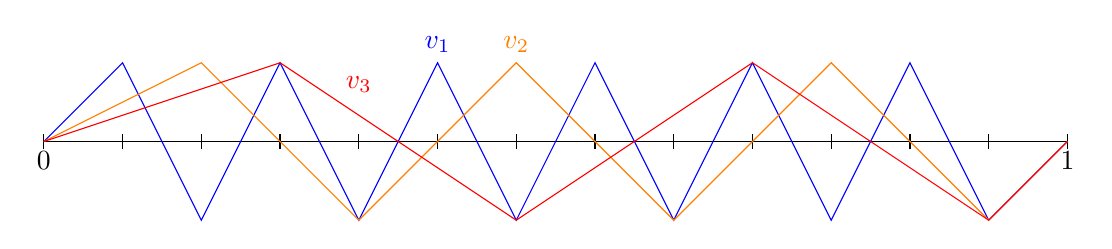
\begin{tikzpicture}
        \draw (0,0) -- (13,0);
        \draw node[below] at (0, 0) {$0$};
        \draw node[below] at (13, 0) {$1$};
        \foreach \i in {0, ..., 13}{
          \draw (\i, -0.1) -- (\i, 0.1);}

        \draw[blue] (0, 0)-- (1, 1) -- (2, -1) -- (3, 1) -- (4, -1)-- (5, 1) -- (6, -1) -- (7, 1)-- (8, -1)-- (9, 1)-- (10, -1)-- (11, 1)-- (12, -1) -- (13, 0) node[above] at (5, 1) {$v_{1}$};
        \draw[orange] (0, 0)-- (2, 1) -- (4, -1) -- (6, 1) -- (8, -1)-- (10, 1) -- (12, -1) -- (13, 0) node[above] at (6, 1) {$v_{2}$};
        \draw[red] (0, 0)-- (3, 1) -- (6, -1) -- (9, 1) -- (12, -1) -- (13, 0) node[above] at (4, 0.5) {$v_{3}$};
      \end{tikzpicture}
      \caption{Skizze zu $v_k$}
      \label{fig:vk}
    \end{figure}
  \end{enumerate}
  Für die Galerkin-Lösung $u_{h}$ gilt
  \begin{align*}
    \nnnorm{u_{h}}^{2}_{\epsilon} \leq a(u_{h}, u_{h}) = (f, u_{h}) \psi \nnorm f _{L_{2}} \nnnorm {u_{h}}_{\epsilon}, 
  \end{align*}
  alsi ist $ \nnnorm {u_{h}}_{\epsilon}$ beschränkt. Kann $v^{k}$ Bestandteil von $u_{h}$ sein? Mit einer direkten Rechnung kann man zeigen, dass
  \begin{align*}
    \nnnorm{v_{k}}_{\epsilon}^{2} \leq C \( \frac \epsilon {h^{2}} + 1\), 
  \end{align*}
  was für kleines $\epsilon$ beschränkt ist. Also: Aus der Stabilität bezüglich der Energienorm kann eine solche Funktion $v^{k}$ nicht ausgeschlossen werden. 

  Aber: Mit $B(k) = \set{v \in V_{h}: \, v(\tilde x_{j}) = 0, \, j = 0, 1, \dots, J}$ als polynomialen Blasenraum und $\Pi_{k}$ als stückweise $L_{2}$-Projektion auf diesem Blasenraum folgt
  \begin{align*}
    \nnorm{\Pi_{k}1}_{0, h}^{2} = \alpha \cdot h
  \end{align*}
  mit von $k$ und $h$ unabhängigen $\alpha$. Sei nun $\delta = \delta_{k}$ konstant. Dann folgt
  \begin{align*}
    \sum_{k} \delta \nnorm{\Pi_{k} v^{k'}}_{L_{2}(k)}^{2} \geq \alpha \delta \nnorm {v_{h}'}_{L_{2}(\tilde x_{1}, \tilde x_{J-1})} = \frac{4 \alpha \delta}{k^{2} h^{2}} (\tilde x_{J-1} - \tilde x_{1}) \geq C h^{-1}, 
  \end{align*}
  ($\delta = h$). Somit können die $v^{k}$ für $k \geq 2$ nicht Bestandteil von $u_{h}$ sein 
  % ($k = 1$: uninteressant, Funktionen, die stückweise linear und in den Gitterpunkten $0$ sind\dots)
  . Nur die hochfrequenten Funktionen $v^{1}$ können Bestandteil sein. 
\end{bemerkung*}

%%% local Variables: 
%%% mode: latex
%%% TeX-master: "vorlesung"
%%% End: 
